\documentclass[12pt,titlepage,a4paper]{article}
\usepackage[utf8]{inputenc}
\usepackage[polish]{babel}
\usepackage{polski}
\usepackage{titling}
\usepackage{vhistory}
\usepackage[margin=2.5cm]{geometry}
\usepackage{graphicx}
\usepackage[parfill]{parskip}
\usepackage{longtable}

\newcommand{\subtitle}[1]{%
  \posttitle{%
    \par\end{center}
    \begin{center}\large#1\end{center}
    \vskip0.5em}%
}

\def\arraystretch{1.5}

\title{System wspomagający pracę firmy kurierskiej}
\subtitle{Specyfikacja wymagań}
\date{}
\author{Jan Tarnowski}


\begin{document}
\maketitle

\begin{versionhistory}
\vhEntry{1.0}{20.06.2014}{Jan Tarnowski}{Pierwsza wersja dokumentu, zrealizowana na podstawie dokumentu wizji.}
\end{versionhistory}

\clearpage
\tableofcontents
\clearpage

\section{Wprowadzenie}

\subsection{Cel dokumentu}
Dokument ten zawiera specyfikację wymagań Systemu Wspomagającego Pracę Firmy Kurierskiej. Został on opracowany na podstawie dokumentu wizji oraz informacji pozyskanych od kierownictwa firmy na temat specyfikowanego systemu.

Uprawnionymi do wglądu w ten dokument są pracownicy Firmy Kurierskiej zaangażowani w powstawanie Systemu Wspomagającego Pracę Firmy Kurierskiej. 

\subsection{Przyjęte zasady w dokumencie}
\subsubsection*{Śledzenie zmian w dokumencie}
Historia zmian dokumentu znajduje się na drugiej stronie dokumentu i jest zrealizowana w formie tabeli. Wpis dotyczący ostatniej zmiany w dokumencie powinien być umieszczony w pierwszym wierszu tabeli i musi zawierać datę zmiany, dane autora zmiany, skrótowy komentarz odnośnie przyczyny zmiany oraz numer kolejnej wersji dokumentu. Numer kolejnej wersji dokumentu jest wyznaczany przez zwiększenie o jeden numeru wersji po kropce (np. 1.01 $\rightarrow$ 1.02) lub w przypadku znaczącej zmiany treści przez zwiększenie o jeden liczby przed kropką i wyzerowanie liczby po kropce (np. 1.05 $\rightarrow$ 2.00).

\subsubsection*{Definiowanie wymagań pozafunkcjonalnych}
Wszystkie wymagania z wyjątkiem wymagań funkcjonalnych będą definiowane za pomocą poniższej tabeli.
\begin{center}
\begin{tabular}[h]{|p{1.6cm}|p{13.5cm}|}
\hline
ID: & Unikalny identyfikator wymagania \\ \hline
Nazwa: & Nazwa wymagania \\ \hline
Priorytet: & Niski / Średni / Wysoki \\ \hline
Opis: & Dokładny opis definiowanego wymagania. \\
\hline
\end{tabular}
\end{center}

\subsubsection*{Definiowanie aktorów}
Aktorzy będą definiowani za pomocą poniższej tabeli.
\begin{center}
\begin{tabular}[h]{|p{1.6cm}|p{13.5cm}|}
\hline
ID: & Unikalny identyfikator aktora z prefiksem ''AKT\_'' \\ \hline
Nazwa: & Nazwa aktora \\ \hline
Opis: & Opis aktora \\
\hline
\end{tabular}
\end{center}

\subsubsection*{Definiowanie obiektów biznesowych}
Obiekty biznesowe będą definiowane za pomocą poniższej tabeli.
\begin{center}
\begin{tabular}[h]{|p{1.6cm}|p{13.5cm}|}
\hline
ID: & Unikalny identyfikator obiektu biznesowego z prefiksem ''OBB\_'' \\ \hline
Nazwa: & Nazwa obiektu biznesowego \\ \hline
Opis: & Opis obiektu biznesowego \\
\hline
\end{tabular}
\end{center}

\subsubsection*{Definiowanie procesów biznesowych oraz scenariuszy przypadków użycia}
Procesy biznesowe oraz scenariusze przypadków użycia będą definiowane za pomocą poniższej tabeli.

\begin{center}
\begin{longtable}[h]{|p{1.6cm}|p{13.5cm}|}
\hline
\textbf{ID:} & Unikalny identyfikator procesu z prefiksem ''PRB\_'' lub identyfikator przypadku użycia z prefiksem ''PUZ\_'' \\ \hline
\textbf{Nazwa:} & Nazwa procesu biznesowego \\ \hline
\multicolumn{2}{|p{15.1cm}|}{\textbf{Aktorzy główni:} ID lub nazwy aktorów głównych biorących udział w procesie} \\
\multicolumn{2}{|p{15.1cm}|}{\textbf{Aktorzy pomocniczy:} ID lub nazwy aktorów pomocniczych biorących udział w procesie} \\
\multicolumn{2}{|p{15.1cm}|}{\textbf{Poziom:}  Biznesowy / Użytkownika / Podfunkcji} \\
\multicolumn{2}{|p{15.1cm}|}{\textbf{Priorytet:}  Niski / Średni / Wysoki} \\
\hline
\multicolumn{2}{|p{15.1cm}|}{\textbf{Opis:}} \\
\multicolumn{2}{|p{15.1cm}|}{Opis procesu biznesowego.
} \\ \hline
\multicolumn{2}{|p{15.1cm}|}{\textbf{Wyzwalacze:}} \\
\multicolumn{2}{|p{15.1cm}|}{Wyszczególnienie zdarzeń wyzwalających proces.
} \\ \hline
\multicolumn{2}{|p{15.1cm}|}{\textbf{Warunki początkowe:}} \\
\multicolumn{2}{|p{15.1cm}|}{Warunki początkowe procesu.
} \\ \hline
\multicolumn{2}{|p{15.1cm}|}{\textbf{Warunki końcowe:}} \\
\multicolumn{2}{|p{15.1cm}|}{Warunki końcowe procesu.
} \\ \hline
\multicolumn{2}{|p{15.1cm}|}{\textbf{Scenariusz główny:}} \\
\multicolumn{2}{|p{15.1cm}|}{Scenariusz główny procesu.
} \\ \hline
\multicolumn{2}{|p{15.1cm}|}{\textbf{Scenariusze alternatywne i rozszerzenia:}} \\
\multicolumn{2}{|p{15.1cm}|}{Scenariusze alternatywne procesu.
} \\ \hline
\multicolumn{2}{|p{15.1cm}|}{\textbf{Wyjątki:}} \\
\multicolumn{2}{|p{15.1cm}|}{Wyjątki procesu.
} \\ \hline
\multicolumn{2}{|p{15.1cm}|}{\textbf{Dodatkowe wymagania:}} \\
\multicolumn{2}{|p{15.1cm}|}{Dodatkowe wymagania procesu.
} \\
\hline
\end{longtable}
\end{center}

\subsubsection*{Definiowanie spraw otwartych}
Sprawy otwarte będą definiowane z wykorzystaniem poniższej tabeli.

\begin{center}
\begin{tabular}[h]{|p{2cm}|p{13.1cm}|}
\hline
ID: & Unikalny identyfikator sprawy otwartej z prefiksem ''SPO\_'' \\ \hline
Nazwa: & Nazwa sprawy otwartej \\ \hline
Opis: & Opis sprawy otwartej. \\
\hline
\end{tabular}
\end{center}

\subsection{Zakres produktu}
Głównym celem projektu jest zbudowanie Systemu Wspomagającego Pracę Firmy Kurierskiej, który będzie miał na celu wsparcie całościowego cyklu życia przesyłki, od momentu nadania przez klienta do czasu dostarczenia jej do odbiorcy. 

System pozwoli na ułatwienie procesu obsługi klienta głównie poprzez zagregowanie informacji o klientach oraz ich przystępną prezentację. Dodatkowo system będzie umożliwiał przeprowadzenie procesu windykacji należności.

Będzie on również wspomagał pracę sortowni, gdzie głównym jego zadaniem będzie optymalizacja procesu dostarczenia paczek oraz ułatwienie rezerwacji transportu międzyregionalnego korzystającego z zewnętrznych pośredników.

System skierowany jest także do klientów firmy, którym umożliwi pozyskiwanie informacji na temat firmy oraz procesu nadawania paczek, a także pozwoli na ich monitorowanie oraz nadawanie.

%W zakres systemu będzie wchodzić aplikacja dla klientów umożliwiająca między innymi monitorowanie statusu wysłanych przez nich przesyłek, nadawanie ich oraz pozyskiwanie potrzebnych informacji o firmie i procesie dostarczania paczek.
%
%Kolejnym zadaniem SWPFK będzie wspomaganie obsługi sortowni, co pozwoli na:
%\begin{itemize}
%\item szeregowanie paczek do wysłania według ich priorytetu oraz miejsca dostarczenia,
%\item rezerwowanie transportu u zewnętrznych pośredników komunikacyjnych obsługujących samoloty oraz pociągi,
%\item rezerwację transportu we własnej flocie międzyregionalnej,
%\item odpowiednie zaplanowanie i rozmieszczenie paczek w samochodach doręczających tak, aby zoptymalizować proces dostarczania.
%\end{itemize}

%System będzie również wspomagał obsługę klienta dostarczając zagregowanych informacji o kliencie wraz z pełną historią interakcji firmy z klientem. Będzie on także obsługiwał proces windykacji należności od klientów.

%który obejmuje swym zakresem:
%\begin{itemize}
%\item Stworzenie aplikacji skierowanej do klientów firmy za pomocą, której %będą oni mogli 
%\end{itemize}

\subsection{Literatura}
\label{subsec:Literatura}
\begin{enumerate}
\item Ustawa z dnia 29 sierpnia 1997 r. o ochronie danych osobowych (Dz.U. 1997 nr 133 poz. 883 z późniejszymi zmianami).
\item Ustawa z dnia 23 listopada 2012 r. Prawo pocztowe (Dz.U. 2012 poz. 1529).
\item Ustawa z dnia 15 listopada 1984 r. Prawo przewozowe (Dz.U. 1984 nr 53 poz. 272 z późniejszymi zmianami).
\item IEEE Standard for Software User Documentation, IEEE Std 1063-2001, 2001.
\end{enumerate}
\section{Opis ogólny}

\subsection{Perspektywa produktu}
System SWPFK ma na celu zastąpienie istniejącego systemu, który jest już przestarzały oraz nie spełnia wymagań firmy kurierskiej. Będzie on funkcjonował jako niezależne oprogramowanie wspomagające szereg procesów związanych z usługami dostarczanymi przez firmę.

System będzie udostępniał \textbf{klientom firmy} interfejs za pomocą, którego będą mogli zamówić odpowiednie usługi oraz uzyskać niezbędne informacje. Interfejs ten powinien być oparty na technologii zapewniającej szeroką dostępność dla klientów firmy.

\textbf{Kurierom} system będzie dostarczał mobilnego rozwiązania wspomagającego proces odbioru i doręczenia przesyłek. Rozwiązanie to będzie zbudowane w oparciu o urządzenia mobilne zapewniające bezprzewodową łączność z systemem.

\textbf{Pracownikom obsługi klienta} system będzie dawał możliwość dostępu do pełnej historii klienta i informacji o nim. Istotne jest aby wykorzystany interfejs zapewniał wysoką przejrzystość prezentowanych danych.

\textbf{Pracownicy sortowni} będą mieli dostęp do interfejsów zapewniających im pomoc w odpowiednim uszeregowaniu przesyłek oraz zaplanowaniu trasy doręczenia aby zmaksymalizować efektywność tych procesów. Wspomniany interfejs powinien zapewniać wysoką wydajność oraz przyjazną wizualizację wyników algorytmu.

System będzie również udostępniał interfejsy umożliwiające integrację z \textbf{systemami zewnętrznych firm} transportowych w celu korzystania z ich usług z poziomu SWPFK.

Rysunek \ref{diag:perspektywa} przedstawia diagram kontekstu dla SWPFK. Zawiera on podstawowych aktorów prowadzących interakcję z systemem oraz podstawowe informacje jakie będą z~nim wymieniać.

\begin{figure}[ht]
	\centering
	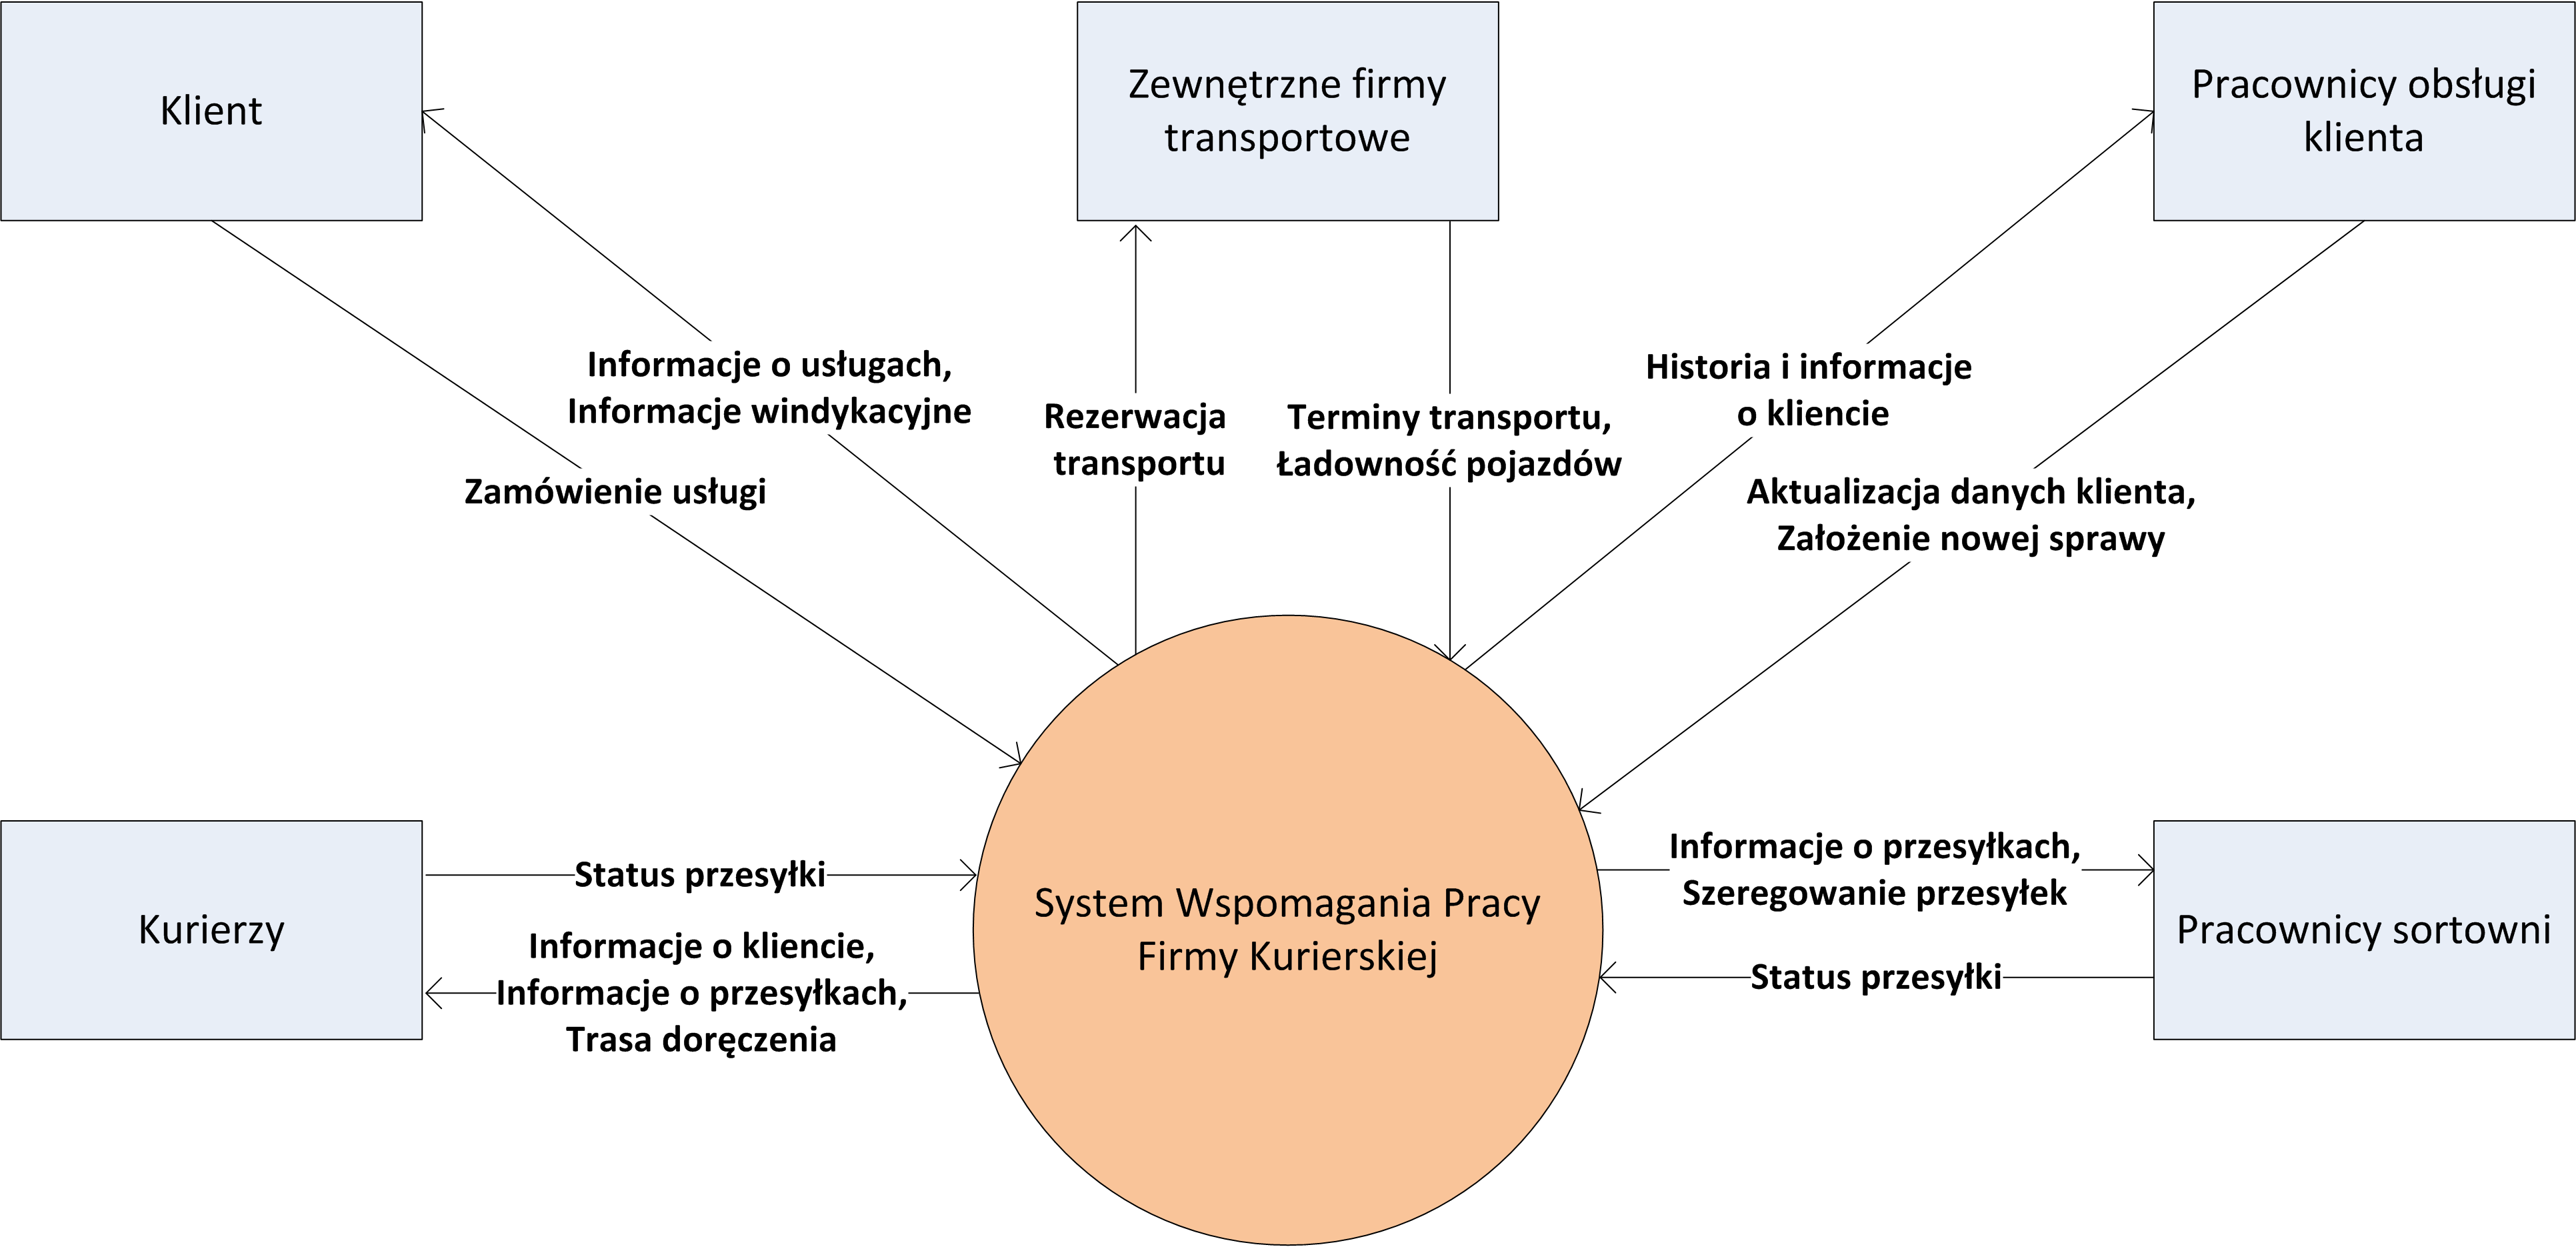
\includegraphics[width=\textwidth]{img/perspektywa}
	\caption{Diagram kontekstu dla SWPFK.}
	\label{diag:perspektywa}
\end{figure}

\subsection{Funkcje produktu}
Podstawową funkcją SWPFK będzie możliwość rejestracji przesyłki w systemie oraz śledzenie jej drogi od momentu nadania do doręczenia. Ponadto pozwoli on na odpowiednie zoptymalizowanie transportu przesyłek oraz wyznaczenie najlepszej drogi ich doręczenia do adresata.

System będzie zapewniał klientom firmy kurierskiej możliwość stałego dostępu do szczegółowych informacji na temat usług świadczonych przez firmę. SWPFK będzie również udostępniał możliwość zamówienia dowolnej usługi za pomocą odpowiednich interfejsów, skorzystania z pomocy obsługi klienta oraz rejestracji klienta w systemie.

Pracownicy obsługi klienta będą używać SWPFK w celu:
\begin{itemize}
\item obsługi klientów w POK;
\item dostępu do przekrojowej informacji o kliencie, która będzie zawierała m. in. jego pełną historię;
\item obsługi klientów kanałem online.
\end{itemize}

System będzie również umożliwiał zamówienie usługi transportu w zewnętrznej firmie transportowej oraz obsługę windykacji w szczególności klientów masowych.

\subsection{Ograniczenia}

\subsubsection{Zgodność z aktami prawnymi}
SWPFK musi być zgodny z rozporządzeniami oraz ustawami wymieniowymi w rozdziale \ref{subsec:Literatura} w punktach 1, 2 oraz 3.

\subsubsection{Zgodność ze standardami i normami}
Dokumentacja użytkownika musi być zgodna ze standardem IEEE 1063-2001 (punkt 4 w rozdziale \ref{subsec:Literatura}).

\subsubsection{System zarządzania bazą danych}
Firma Kurierska posiada 4 licencje na bazę danych firmy Oracle w wersji 10g z możliwością aktualizacji do wersji 11g. Licencje są w wersji Enterprise Edition oraz typu procesorowego co pozwala na użytkowanie bazy przez wielu użytkowników. Do licencji zostało również wykupione wsparcie na wypadek wystąpienia problemów w obsłudze bazy danych.

Ze względu na posiadane licencje SWPFK powinien być zbudowany w oparciu o bazę danych firmy Oracle. SWPFK będzie agregował duże ilości danych dotychczas rozproszonych po odseparowanych systemach co może skutkować koniecznością dokupienia większej ilości licencji, aby móc zainstalować system na sprzęcie o większej mocy obliczeniowej.

Wykorzystanie posiadanych licencji pozwoli na obniżenie kosztów systemu oraz zaangażowanie dotychczas zdobytego doświadczenia w obsłudze baz danych Oracle.

\subsubsection{Ograniczenia sprzętowe}
\subsubsection*{Infrastruktura sieciowa}
Moduł serwerowy SWPFK będzie uruchomiony w jednej fizycznej lokalizacji. Z tego względu wymaga się, aby serwerownia w której będzie uruchomiony moduł serwerowy SWPFK miała zapewnione co najmniej dwa redundantne połączenia światłowodowe do sieci Internet. Każde z tych połączeń powinno pochodzić od innego ISP oraz charakteryzować się przepustowością na poziomie co najmniej 10 Gb/s. Ponadto każde z połączeń musi zapewniać dostępność na poziomie minimum 99,999\% w~skali miesiąca.

Ponadto połączenia sieciowe między dowolnymi dwoma elementami serwerowni powinny charakteryzować się przepustowością co najmniej 10 Gb/s.

\subsubsection*{Konfiguracja sprzętowa serwera}
Wymaga się aby moduł serwerowy SWPFK był w stanie obsłużyć jednocześnie  do 10000 równoległych sesji użytkowników korzystających z interfejsu internetowego oraz prowadzić obsługę innych aplikacji SWPFK spełniając wszystkie stawiane przed SWPFK wymagania wydajnościowe. 

W celu spełnienia wymagań niezawodności SWPFK powinien być uruchomiony na dwóch niezależnych serwerach, z których jeden będzie pełnił funkcję zapasową i przejmie obsługę SWPFK tylko w sytuacji awarii głównej instancji.

W poniższej tabeli znajduje się minimalna konfiguracja serwera obsługującego moduł serwerowy SWPFK.

\begin{center}
\begin{tabular}[h]{|p{3.5cm}|p{11.6cm}|}
\hline
Procesory: & 16 procesorów 12-wątkowych o częstotliwości taktowania zegara 2,5 GHz i 15 MB pamięci podręcznej, np. Intel E5-2630 v2 lub inny o nie niższej mocy obliczeniowej\\ \hline
Pamięć RAM: & 512 GB \\ \hline
Karta sieciowa: & Dwie karty sieciowe każda o przepustowości 10 Gb/s \\ \hline
Pojemność dyskowa & Efektywnie 10 TB, dyski działające w macierzy typu RAID 5 \\ \hline
System operacyjny: & SUSE Linux Enterprise Server 11 \\ \hline
Dodatkowe oprogramowanie: & Java w wersji co najmniej 1.7 \\
\hline
\end{tabular}
\end{center}

\subsubsection*{Stacja robocza dla aplikacji klienckiej}
Minimalne wymagania aplikacji klienckiej SWPFK do poprawnego działania na stacji roboczej przedstawia poniższa tabela.

\begin{center}
\begin{tabular}[h]{|p{3.5cm}|p{11.6cm}|}
\hline
Procesor: & Intel Core i3 1,8 GHz lub inny o zbliżonej mocy obliczeniowej \\ \hline
Pamięć RAM: & 1,5 GB \\ \hline
Karta sieciowa: & 100Mb/s \\ \hline
Dostępna pojemność dysku: & 1,5 GB \\ \hline
System operacyjny: & Windows Vista \\ \hline
Dodatkowe oprogramowanie: & Microsoft .NET Framework 3.5 \\
\hline
\end{tabular}
\end{center}

\subsubsection{Protokoły komunikacyjne}
SWPFK powinien wykorzystywać w komunikacji jedynie otwarte protokoły komunikacyjne sieci Internet.

\subsubsection{Instalacja oprogramowania}
Aplikacja kliencka instalowana na komputerach PC nie powinna wymagać praw administratora aby zostać zainstalowana. Ponadto instalator aplikacji klienckiej powinien być dystrybuowany w postaci pojedynczego, niezależnego pliku. Plik ten po uruchomieniu powinien przeprowadzić użytkownika przez proces instalacji w formie czytelnego kreatora. Zakłada się, że do instalacji użytkownik nie będzie potrzebował żadnej specjalistycznej wiedzy z zakresu obsługi komputerów.

Aplikacja mobilna będzie instalowana na terminalach mobilnych przez wyspecjalizowanych techników. Również moduł serwerowy będzie instalowany na serwerze przez osoby posiadające zaawansowaną wiedzę z zakresu utrzymywania i instalacji oprogramowania serwerowego.

\subsubsection{Interfejsy programistyczne}
Wszystkie moduły SWPFK powinny implementować interfejsy programistyczne tak aby były one możliwe do osiągnięcia za pomocą technologii Java oraz .NET Framework bez ponoszenia kosztów implementacji własnych bibliotek obsługujących niestandardowe rozwiązanie.

\subsection{Dokumentacja użytkownika}
Dokumentacja SWPFK będzie się składać z:
\begin{center}
\begin{tabular}[h]{|p{2cm}|p{13.1cm}|}
\hline
Nazwa: & Dokumentacja techniczna SWPFK \\ \hline
Opis: & Dokument będzie opisywał architekturę wszystkich modułów SWPFK, zastosowane technologie i rozwiązania oraz instrukcje instalacji i utrzymania każdego modułu. \\ \hline
Standard: & IEEE 1063-2001 \\ \hline
Format: & elektroniczny (w formie pliku PDF), drukowany \\ \hline
Język: & angielski \\
\hline
\end{tabular}
\end{center}

\begin{center}
\begin{tabular}[h]{|p{2cm}|p{13.1cm}|}
\hline
Nazwa: & Przewodnik użytkownika aplikacji klienckiej \\ \hline
Opis: & Dokument będzie zawierał szczegółowy opis wszystkich dostępnych  funkcjonalności aplikacji klienckiej. Będzie również zawierał opis każdego okna aplikacji. \\ \hline
Standard: & IEEE 1063-2001 \\ \hline
Format: & elektroniczny (w formie pliku PDF), drukowany \\ \hline
Język: & polski, angielski, niemiecki, hiszpański, francuski, czeski, słowacki \\
\hline
\end{tabular}
\end{center}

\begin{center}
\begin{tabular}[h]{|p{2cm}|p{13.1cm}|}
\hline
Nazwa: & Przewodnik użytkownika aplikacji mobilnej \\ \hline
Opis: & Dokument będzie zawierał szczegółowy opis wszystkich dostępnych  funkcjonalności aplikacji mobilnej oraz sposób ich użycia.  \\ \hline
Standard: & IEEE 1063-2001 \\ \hline
Format: & elektroniczny (w formie pliku PDF), drukowany \\ \hline
Język: & polski, angielski, niemiecki, hiszpański, francuski, czeski, słowacki \\
\hline
\end{tabular}
\end{center}

\subsection{Założenia i zależności}
Zakłada się, że użytkownik interfejsu internetowego SWPFK będzie korzystał z jednej z poniższych przeglądarek internetowych:
\begin{enumerate}
\item Internet Explorer 10, 11;
\item Mozilla Firefox w wersji co najmniej 28;
\item Google Chrome w wersji 35 lub wyższej;
\item Apple Safari w wersji co najmniej 5.
\end{enumerate}

Zakłada się, że użytkownicy aplikacji klienckiej na komputer PC będą korzystać z systemu Microsoft Windows Vista lub jego nowszej wersji. Ponadto użytkownicy będą mieli zainstalowane oprogramowanie Microsoft .NET Framework w wersji co najmniej 3.5.
\section{Model procesów biznesowych}

\subsection{Aktorzy i charakterystyka użytkowników}
\begin{center}
\begin{tabular}[h]{|p{1.6cm}|p{13.5cm}|}
\hline
ID: & AKT\_KLIENT \\ \hline
Nazwa: & Klient \\ \hline
Opis: & Klient to osoba sporadycznie korzystająca z usług Firmy Kurierskiej, np. poprzez jednorazowe nadanie przesyłki. Nie posiada stałego związku z firmą. Korzysta on z SWPFK za pomocą interfejsu internetowego, którego używa do pozyskania informacji o interesujących go usługach oraz za pośrednictwem pracownika POK. \\
\hline
\end{tabular}
\end{center}

\begin{center}
\begin{tabular}[h]{|p{1.6cm}|p{13.5cm}|}
\hline
ID: & AKT\_KLIENT\_BIZ \\ \hline
Nazwa: & Klient biznesowy \\ \hline
Opis: & Klient biznesowy to osoba lub podmiot prawny posiadający podpisaną umowę z Firmą Kurierską na świadczenie usług przewozowych. Często i regularnie korzysta z usług firmy. Korzysta z interfejsu internetowego SWPFK, oraz posiada własne konto w SWPFK.  \\
\hline
\end{tabular}
\end{center}

\begin{center}
\begin{tabular}[h]{|p{1.6cm}|p{13.5cm}|}
\hline
ID: & AKT\_ODBIORCA \\ \hline
Nazwa: & Odbiorca przesyłki \\ \hline
Opis: & Odbiorca przesyłki to osoba do której klient firmy nadał przesyłkę. Przesyłka ta jest dostarczana do odbiorcy za pomocą kuriera. Korzysta on z SWPFK w celu sprawdzenia aktualnego statusu przesyłki. \\
\hline
\end{tabular}
\end{center}

\begin{center}
\begin{tabular}[h]{|p{1.6cm}|p{13.5cm}|}
\hline
ID: & AKT\_PRAC\_PKT\_OBS\_KL \\ \hline
Nazwa: & Pracownik punktu obsługi klienta \\ \hline
Opis: & Pracownik punktu obsługi klienta jest pracownikiem Firmy Kurierskiej lub osobą która świadczy usługi w imieniu i na licencji Firmy Kurierskiej. Jego praca polega na przyjmowaniu oraz wydawaniu przesyłek w stacjonarnych POK rozmieszczonych poza siedzibą firmy. Dodatkowo jego zadaniem jest udzielanie informacji dotyczących usług firmy. Posiada indywidualne konto w SWPFK i ma do niego dostęp za pomocą aplikacji klienckiej. \\
\hline
\end{tabular}
\end{center}

\begin{center}
\begin{tabular}[h]{|p{1.6cm}|p{13.5cm}|}
\hline
ID: & AKT\_PRAC\_SORT \\ \hline
Nazwa: & Pracownik sortowni \\ \hline
Opis: & Pracownik sortowni jest pracownikiem Firmy Kurierskiej w jednej z sortowni firmy. Jego zadanie polega na identyfikowaniu przesyłek oraz prowadzeniu załadunku pojazdów transportujących przesyłki do kolejnych sortowni lub do odbiorcy. \\
\hline
\end{tabular}
\end{center}

\begin{center}
\begin{tabular}[h]{|p{1.6cm}|p{13.5cm}|}
\hline
ID: & AKT\_KURIER \\ \hline
Nazwa: & Kurier \\ \hline
Opis: & Kurier to pracownik Firmy Kurierskiej, który zajmuje się odbieraniem od oraz dostarczaniem przesyłek bezpośrednio do odbiorcy. Uzyskuje dostęp do SWPFK za pomocą terminalu mobilnego. Używa SWPFK w celu uzyskania informacji o danych adresowych odbiorcy przesyłki, wyliczenia najbardziej optymalnej trasy przejazdu podczas doręczenia oraz do identyfikacji przesyłek. \\
\hline
\end{tabular}
\end{center}

\begin{center}
\begin{tabular}[h]{|p{1.6cm}|p{13.5cm}|}
\hline
ID: & AKT\_PRAC\_OBS\_KL \\ \hline
Nazwa: & Pracownik obsługi klienta \\ \hline
Opis: & Pracownik obsługi klienta to pracownik Firmy Kurierskiej. Obsługuje on klientów firmy, dostarczając im pomocy w rozwiązaniu problemów związanych z usługami firmy. Pomoc ta jest świadczona poprzez interfejs internetowy SWPFK oraz telefon. Zajmuje się on także sprawami związanymi z wystawianiem faktur za usługi oraz windykacją. \\
\hline
\end{tabular}
\end{center}

\begin{center}
\begin{tabular}[h]{|p{1.6cm}|p{13.5cm}|}
\hline
ID: & AKT\_ZEWN\_FIR\_TRANSP \\ \hline
Nazwa: & Zewnętrzna firma transportowa \\ \hline
Opis: & Zewnętrzna firma transportowa to podmiot całkowicie odrębny od Firmy Kurierskiej. Świadczy ona usługi transportu towarów posiadanymi przez siebie środkami transportu (np. pociąg, samolot). SWPFK integruje się z jej systemem w celu umożliwienia użytkownikom zamówienia usług firmy z bezpośrednio poziomu interfejsu SWPFK. \\
\hline
\end{tabular}
\end{center}

\subsection{Obiekty biznesowe}
Poniżej zostały wyszczególnione najważniejsze obiekty biznesowe występujące w SWPFK.

\begin{center}
\begin{tabular}[h]{|p{1.6cm}|p{13.5cm}|}
\hline
ID: & OBB\_PRZESYLKA \\ \hline
Nazwa: & Przesyłka \\ \hline
Opis: & Obiekt przekazany przez klienta Firmie Kurierskiej w celu przetransportowania go do wskazanego odbiorcy. Przesyłka posiada unikalny w skali SWPFK identyfikator, który pozwala jednoznacznie ją zidentyfikować. Przesyłkę charakteryzuje jej waga, wymiary oraz priorytet dostarczenia. Priorytet przesyłki zależy od wskazanej zawartości lub jest określany bezpośrednio przez klienta. \\
\hline
\end{tabular}
\end{center}

\begin{center}
\begin{tabular}[h]{|p{1.6cm}|p{13.5cm}|}
\hline
ID: & OBB\_KLIENT \\ \hline
Nazwa: & Klient \\ \hline
Opis: & Jest to tożsamość aktorów AKT\_KLIENT oraz AKT\_KLIENT\_BIZ pozwalająca na ich identyfikację w Firmie Kurierskiej. Obiekt Klient posiada unikalny w skali SWPFK identyfikator, który pozwala na powiązanie go z innymi obiektami w systemie. Obiekt zawiera również dowiązania do innych tożsamości tego klienta w odrębnych systemach działających w obrębie Firmy Kurierskiej. \\
\hline
\end{tabular}
\end{center}

\begin{center}
\begin{tabular}[h]{|p{1.6cm}|p{13.5cm}|}
\hline
ID: & OBB\_AKTYWNOSC \\ \hline
Nazwa: & Aktywność klienta \\ \hline
Opis: & Jest to zapis interakcji pracownika Firmy Kurierskiej z klientem lub zlecenia/pracy realizowanej dla konkretnego klienta . Zawiera dane takie jak czas, miejsce i opis wydarzenia. Jeśli nie narusza to obowiązującego prawa aktywność posiada także pełny zapis przebiegu interakcji, np. kopie korespondencji.  \\
\hline
\end{tabular}
\end{center}

\begin{center}
\begin{tabular}[h]{|p{1.6cm}|p{13.5cm}|}
\hline
ID: & OBB\_FAKTURA \\ \hline
Nazwa: & Faktura \\ \hline
Opis: & Dokument zawierający szczegółowe zestawienie kosztów za usługi wykonane dla konkretnego klienta. Jest on ściśle powiązany z klientem i zawiera jego identyfikator. Klient na podstawie faktury jest zobowiązany do uregulowania należności wobec Firmy Kurierskiej we wskazanej kwocie oraz we wskazanym terminie. \\
\hline
\end{tabular}
\end{center}

\begin{center}
\begin{tabular}[h]{|p{1.6cm}|p{13.5cm}|}
\hline
ID: & OBB\_UMOWA \\ \hline
Nazwa: & Umowa \\ \hline
Opis: & Dokument zawarty pomiędzy aktorem AKT\_KLIENT\_BIZ a Firmą Kurierską, który określa zasady współpracy tych dwóch podmiotów. Dotyczy ona ustalenia preferencyjnych warunków świadczenia usług klientowi np. w zamian za regularne korzystanie z usług firmy. Zawiera ona unikalny w skali systemu identyfikator oraz dowiązanie do obiektu klienta. \\
\hline
\end{tabular}
\end{center}

\begin{center}
\begin{tabular}[h]{|p{1.6cm}|p{13.5cm}|}
\hline
ID: & OBB\_ZLECENIE \\ \hline
Nazwa: & Zlecenie \\ \hline
Opis: & Jest to zamówienie przez klienta wykonania usługi świdczonej przez Firmę Kurierską. Otrzymuje ono unikalny identyfikator i jest ściśle powiązane z konkretnym klientem firmy. Zawiera informacje o rodzaju usługi, czasie zamówienia i wykonania, miejscy zamówienia i wykonania oraz przydzielonych zasobach do realizacji usługi. Po zrealizowaniu usługi jej przebieg jest archiwizowany w postaci obiektu OBB\_AKTYWNOSC. \\
\hline
\end{tabular}
\end{center}

\begin{center}
\begin{tabular}[h]{|p{1.6cm}|p{13.5cm}|}
\hline
ID: & OBB\_POJAZD \\ \hline
Nazwa: & Pojazd transportowy \\ \hline
Opis: & Jest to pojazd będący w posiadaniu Firmy Kurierskiej lub możliwy do wynajęcia od zewnętrznej firmy transportowej służący do transportu przesyłek pomiędzy sortowniami firmy oraz bezpośrednio do klienta. Posiada swój unikalny identyfikator oraz charakteryzują go takie dane jak: ładowność oraz wymiary części załadunkowej. \\
\hline
\end{tabular}
\end{center}

\subsection{Procesy biznesowe}
\begin{center}
\begin{longtable}[h]{|p{1.6cm}|p{13.5cm}|}
\hline
\textbf{ID:} & PRB\_ZAM\_ODB\_PRZESYLKI \\ \hline
\textbf{Nazwa:} & Zamówienie odbioru przesyłki przez klienta \\ \hline
\multicolumn{2}{|p{15.1cm}|}{\textbf{Aktorzy główni:}  Klient biznesowy} \\
\multicolumn{2}{|p{15.1cm}|}{\textbf{Aktorzy pomocniczy:}  \textit{Kurier}} \\
\multicolumn{2}{|p{15.1cm}|}{\textbf{Poziom:}  Biznesowy} \\
\multicolumn{2}{|p{15.1cm}|}{\textbf{Priorytet:}  Wysoki} \\
\hline
\multicolumn{2}{|p{15.1cm}|}{\textbf{Opis:}} \\
\multicolumn{2}{|p{15.1cm}|}{Klient biznesowy zleca odbiór przesyłek przez kuriera.
} \\ \hline
\multicolumn{2}{|p{15.1cm}|}{\textbf{Wyzwalacze:}} \\
\multicolumn{2}{|p{15.1cm}|}{1. Klient biznesowy chce nadać przesyłki.
} \\ \hline
\multicolumn{2}{|p{15.1cm}|}{\textbf{Warunki początkowe:}} \\
\multicolumn{2}{|p{15.1cm}|}{
1. Klient biznesowy posiada ważna umowę z Firmą Kurierską na świadczenie usług. \newline
2. Klient jest zalogowany w systemie.
} \\ \hline
\multicolumn{2}{|p{15.1cm}|}{\textbf{Warunki końcowe:}} \\
\multicolumn{2}{|p{15.1cm}|}{
Zlecenie odbioru zostaje utworzone oraz przydzielone kurierowi. Zostają wygenerowane nowe numery paczek w systemie.
} \\ \hline
\multicolumn{2}{|p{15.1cm}|}{\textbf{Scenariusz główny:}} \\
\multicolumn{2}{|p{15.1cm}|}{
\begin{enumerate}
\item Klient biznesowy wprowadza do systemu dane: miejsce odbioru, proponowany czas odbioru, ilość przesyłek, przybliżoną wagę oraz wymiary każdej z przesyłek. \label{sce:wpr_dan}
\item System sprawdza poprawność wprowadzonych danych.
\item System wyznacza możliwy czas odbioru paczek na podstawie proponowanego czasu. \label{sce:wyzn_czas}
\item Klient biznesowy zatwierdza datę odbioru zaproponowaną przez system.
\item System zapisuje zlecenie odbioru i przydziela zlecenie odbioru odpowiedniemu kurierowi.
\item System generuje unikalny numer dla każdej paczki i nadaje im status ''Nie odebrane od nadawcy''.
\item Klient biznesowy oznacza paczki wygenerowanymi numerami.
\end{enumerate}
} \\ \hline
\multicolumn{2}{|p{15.1cm}|}{\textbf{Scenariusze alternatywne i rozszerzenia:}} \\
\multicolumn{2}{|p{15.1cm}|}{
2.a Wprowadzone dane są niepoprawne. \newline
2.a.1 System prezentuje ostrzeżenie o niepoprawnych danych. \newline
2.a.2 Powrót do punktu \ref{sce:wpr_dan} scenariusza głównego. \newline
\newline
4.a Wyznaczony przez system czas odbioru jest nieodpowiedni dla klienta biznesowego. \newline
4.a.1 Klient biznesowy wprowadza inny proponowany czas odbioru przesyłki. \newline
4.a.2 Powrót do punktu \ref{sce:wyzn_czas} scenariusza głównego.
} 
\\ \hline
\multicolumn{2}{|p{15.1cm}|}{\textbf{Wyjątki:}} \\
\multicolumn{2}{|p{15.1cm}|}{
\textit{brak}
} \\ \hline
\multicolumn{2}{|p{15.1cm}|}{\textbf{Dodatkowe wymagania:}} \\
\multicolumn{2}{|p{15.1cm}|}{\textit{brak}
} \\
\hline
\end{longtable}
\end{center}

\begin{center}
\begin{longtable}[h]{|p{1.6cm}|p{13.5cm}|}
\hline
\textbf{ID:} & PRB\_ODBIOR\_PRZESYLEK \\ \hline
\textbf{Nazwa:} & Odbiór przesyłek od klienta biznesowego przez kuriera \\ \hline
\multicolumn{2}{|p{15.1cm}|}{\textbf{Aktorzy główni:}  Klient biznesowy, Kurier} \\
\multicolumn{2}{|p{15.1cm}|}{\textbf{Aktorzy pomocniczy:} \textit{brak}} \\
\multicolumn{2}{|p{15.1cm}|}{\textbf{Poziom:}  Biznesowy} \\
\multicolumn{2}{|p{15.1cm}|}{\textbf{Priorytet:}  Wysoki} \\
\hline
\multicolumn{2}{|p{15.1cm}|}{\textbf{Opis:}} \\
\multicolumn{2}{|p{15.1cm}|}{Kurier odbiera przesyłki od klienta, który wcześniej zamówił odbiór.
} \\ \hline
\multicolumn{2}{|p{15.1cm}|}{\textbf{Wyzwalacze:}} \\
\multicolumn{2}{|p{15.1cm}|}{1. Nadeszła wyznaczona data odbioru przesyłek.
} \\ \hline
\multicolumn{2}{|p{15.1cm}|}{\textbf{Warunki początkowe:}} \\
\multicolumn{2}{|p{15.1cm}|}{Klient biznesowy złożył zlecenie odbioru paczek.
} \\ \hline
\multicolumn{2}{|p{15.1cm}|}{\textbf{Warunki końcowe:}} \\
\multicolumn{2}{|p{15.1cm}|}{
Paczki zostają przekazane kurierowi oraz ich status w systemie zmienia się na ''Odebrana od klienta''.
} \\ \hline
\multicolumn{2}{|p{15.1cm}|}{\textbf{Scenariusz główny:}} \\
\multicolumn{2}{|p{15.1cm}|}{
\begin{enumerate}
\item Klient biznesowy wydaje przesyłki kurierowi. \label{sce:wyd_pacz}
\item Kurier identyfikuje przekazywane przesyłki na podstawie znajdującego się na nich numeru.
\item Kurier wprowadza przesyłki do systemu skanując ich kod za pomocą terminalu mobilnego.
\item System zmienia status paczki na ''Odebrana od klienta''.
\item Kurier generuje oraz podpisuje protokół odbioru przesyłek i przekazuje go klientowi.
\end{enumerate}
} \\ \hline
\multicolumn{2}{|p{15.1cm}|}{\textbf{Scenariusze alternatywne i rozszerzenia:}} \\
\multicolumn{2}{|p{15.1cm}|}{
2.a Przesyłki nie posiadają oznaczeń z numerem. \newline
2.a.1 Kurier odmawia przyjęcia przesyłek. \newline
2.a.2 Klient uzupełnia oznaczenia na przesyłkach. \newline
2.a.3 Powrót do punktu \ref{sce:wyd_pacz} scenariusza głównego. \newline
\newline
3.a Numery przesyłek są niepoprawne lub nieaktualne. \newline
3.a.1 Kurier odmawia przyjęcia przesyłek. \newline
3.a.2 Proces kończy się.
} \\ \hline
\multicolumn{2}{|p{15.1cm}|}{\textbf{Wyjątki:}} \\
\multicolumn{2}{|p{15.1cm}|}{
Terminal mobilny kuriera jest uszkodzony lub nie ma połączenia z systemem.
} \\ \hline
\multicolumn{2}{|p{15.1cm}|}{\textbf{Dodatkowe wymagania:}} \\
\multicolumn{2}{|p{15.1cm}|}{\textit{brak}
} \\
\hline
\end{longtable}
\end{center}

\begin{center}
\begin{longtable}[h]{|p{1.6cm}|p{13.5cm}|}
\hline
\textbf{ID:} & PRB\_DOR\_PRZESYLEK \\ \hline
\textbf{Nazwa:} & Doręczenie przesyłek do odbiorcy \\ \hline
\multicolumn{2}{|p{15.1cm}|}{\textbf{Aktorzy główni:}  Odbiorca, Kurier} \\
\multicolumn{2}{|p{15.1cm}|}{\textbf{Aktorzy pomocniczy:}  \textit{brak}} \\
\multicolumn{2}{|p{15.1cm}|}{\textbf{Poziom:}  Biznesowy} \\
\multicolumn{2}{|p{15.1cm}|}{\textbf{Priorytet:}  Wysoki} \\
\hline
\multicolumn{2}{|p{15.1cm}|}{\textbf{Opis:}} \\
\multicolumn{2}{|p{15.1cm}|}{Kurier wydaje przesyłkę Odbiorcy.
} \\ \hline
\multicolumn{2}{|p{15.1cm}|}{\textbf{Wyzwalacze:}} \\
\multicolumn{2}{|p{15.1cm}|}{
1. Przesyłka dotarła do sortowni najbliższej miejscu doręczenia.
} \\ \hline
\multicolumn{2}{|p{15.1cm}|}{\textbf{Warunki początkowe:}} \\
\multicolumn{2}{|p{15.1cm}|}{
Kurier ustalił z Odbiorcą termin odbioru.
} \\ \hline
\multicolumn{2}{|p{15.1cm}|}{\textbf{Warunki końcowe:}} \\
\multicolumn{2}{|p{15.1cm}|}{
Przesyłka zostaje odebrana i jej status w systemie zostaje zmieniony na ''Doręczona''.
} \\ \hline
\multicolumn{2}{|p{15.1cm}|}{\textbf{Scenariusz główny:}} \\
\multicolumn{2}{|p{15.1cm}|}{
\begin{enumerate}
\item Kurier identyfikuje przesyłki Odbiorcy za pomocą terminala mobilnego.
\item Odbiorca sprawdza stan wydawanych przesyłek.
\item Odbiorca potwierdza odbiór przesyłek składając podpis za pomocą terminala mobilnego.
\item System zmienia status przesyłek na ''Doręczona''.
\item Kurier przekazuje przesyłki Odbiorcy.
\end{enumerate}
} \\ \hline
\multicolumn{2}{|p{15.1cm}|}{\textbf{Scenariusze alternatywne i rozszerzenia:}} \\
\multicolumn{2}{|p{15.1cm}|}{
2.a Odbiorca ma zastrzeżenia do stanu paczek. \newline
2.a.1 Kurier generuje protokół reklamacji w dwóch egzemplarzach. \newline
2.a.2 Odbiorca uzupełnia protokół wprowadzając opis swoich zastrzeżeń. \newline
2.a.3 Odbiorca oraz kurier potwierdzają podpisem zgodność protokołów. \newline
2.a.4 Kurier przekazuje jeden egzemplarz protokołu Odbiorcy. \newline
2.a.5 Proces kończy się.
} \\ \hline
\multicolumn{2}{|p{15.1cm}|}{\textbf{Wyjątki:}} \\
\multicolumn{2}{|p{15.1cm}|}{
Terminal mobilny kuriera jest uszkodzony.
} \\ \hline
\multicolumn{2}{|p{15.1cm}|}{\textbf{Dodatkowe wymagania:}} \\
\multicolumn{2}{|p{15.1cm}|}{
\textit{brak}
} \\
\hline
\end{longtable}
\end{center}

\begin{center}
\begin{longtable}[h]{|p{1.6cm}|p{13.5cm}|}
\hline
\textbf{ID:} & PRB\_UTW\_FAKTURY \\ \hline
\textbf{Nazwa:} & Utworzenie faktury za usługi \\ \hline
\multicolumn{2}{|p{15.1cm}|}{\textbf{Aktorzy główni:} Klient biznesowy} \\
\multicolumn{2}{|p{15.1cm}|}{\textbf{Aktorzy pomocniczy:} } \\
\multicolumn{2}{|p{15.1cm}|}{\textbf{Poziom:}  Biznesowy} \\
\multicolumn{2}{|p{15.1cm}|}{\textbf{Priorytet:}  Wysoki} \\
\hline
\multicolumn{2}{|p{15.1cm}|}{\textbf{Opis:}} \\
\multicolumn{2}{|p{15.1cm}|}{
Klient biznesowy chce otrzymać fakturę za wykonane dla niego usługi.
} \\ \hline
\multicolumn{2}{|p{15.1cm}|}{\textbf{Wyzwalacze:}} \\
\multicolumn{2}{|p{15.1cm}|}{
1. Prośba klienta o wystawienie faktury. \newline
2. Upłynięcie czasu maksymalnego spłaty zaległych należności.
} \\ \hline
\multicolumn{2}{|p{15.1cm}|}{\textbf{Warunki początkowe:}} \\
\multicolumn{2}{|p{15.1cm}|}{
Klient biznesowy jest zalogowany w systemie.
} \\ \hline
\multicolumn{2}{|p{15.1cm}|}{\textbf{Warunki końcowe:}} \\
\multicolumn{2}{|p{15.1cm}|}{
Klient biznesowy otrzymuje fakturę za usługi.
} \\ \hline
\multicolumn{2}{|p{15.1cm}|}{\textbf{Scenariusz główny:}} \\
\multicolumn{2}{|p{15.1cm}|}{
\begin{enumerate}
\item Klient biznesowy wskazuje usługi za które chce otrzymać fakturę.
\item System pobiera dane klienta. \label{sec:pobra_dan_kl}
\item System generuje fakturę na podstawie wskazanych usługi pobranych danych klienta.
\item Faktura jest udostępniana klientowi biznesowemu do pobrania.
\end{enumerate}
} \\ \hline
\multicolumn{2}{|p{15.1cm}|}{\textbf{Scenariusze alternatywne i rozszerzenia:}} \\
\multicolumn{2}{|p{15.1cm}|}{
1.a Klient posiada przedawnione nieopłacone usługi. \newline
1.a.1 System dodaje te usługi do wskazanych przez klienta. \newline
1.a.2 Powrót do punktu \ref{sec:pobra_dan_kl} scenariusza głównego.
} \\ \hline
\multicolumn{2}{|p{15.1cm}|}{\textbf{Wyjątki:}} \\
\multicolumn{2}{|p{15.1cm}|}{
\textit{brak}
} \\ \hline
\multicolumn{2}{|p{15.1cm}|}{\textbf{Dodatkowe wymagania:}} \\
\multicolumn{2}{|p{15.1cm}|}{
\textit{brak}
} \\
\hline
\end{longtable}
\end{center}

\begin{center}
\begin{longtable}[h]{|p{1.6cm}|p{13.5cm}|}
\hline
\textbf{ID:} & PRB\_NAD\_PRZESYLKI\_POK \\ \hline
\textbf{Nazwa:} & Nadanie przesyłki w POK \\ \hline
\multicolumn{2}{|p{15.1cm}|}{\textbf{Aktorzy główni:}  Klient, Pracownik punktu obsługi klienta} \\
\multicolumn{2}{|p{15.1cm}|}{\textbf{Aktorzy pomocniczy:} \textit{brak}} \\
\multicolumn{2}{|p{15.1cm}|}{\textbf{Poziom:}  Biznesowy} \\
\multicolumn{2}{|p{15.1cm}|}{\textbf{Priorytet:}  Średni} \\
\hline
\multicolumn{2}{|p{15.1cm}|}{\textbf{Opis:}} \\
\multicolumn{2}{|p{15.1cm}|}{
Klient chce nadać przesyłkę w POK.
} \\ \hline
\multicolumn{2}{|p{15.1cm}|}{\textbf{Wyzwalacze:}} \\
\multicolumn{2}{|p{15.1cm}|}{
Przyjście klienta z przesyłką do POK.
} \\ \hline
\multicolumn{2}{|p{15.1cm}|}{\textbf{Warunki początkowe:}} \\
\multicolumn{2}{|p{15.1cm}|}{
Pracownik POK jest zalogowany do systemu za pomocą aplikacji klienckiej.
} \\ \hline
\multicolumn{2}{|p{15.1cm}|}{\textbf{Warunki końcowe:}} \\
\multicolumn{2}{|p{15.1cm}|}{
Przesyłce zostaje nadany numer i zostaje ona przekazana pracownikowi POK.
} \\ \hline
\multicolumn{2}{|p{15.1cm}|}{\textbf{Scenariusz główny:}} \\
\multicolumn{2}{|p{15.1cm}|}{
\begin{enumerate}
\item Klient podaje swoje dane adresowe oraz dane odbiorcy pracownikowi POK. \label{sce:kl_pod_dane_pok}
\item System sprawdza poprawność podanych danych.
\item Pracownik POK dokonuje pomiarów parametrów przesyłki.
\item Pracownik POK wprowadza dane przesyłki do systemu.
\item System nadaje przesyłce unikalny numer.
\item Pracownik POK oznacza przesyłkę wygenerowanym numerem.
\item Klient opłaca wybrany typ usługi.
\item Pracownik POK generuje z systemu potwierdzenie nadania przesyłki oraz przekazuje je klientowi.
\end{enumerate}
} \\ \hline
\multicolumn{2}{|p{15.1cm}|}{\textbf{Scenariusze alternatywne i rozszerzenia:}} \\
\multicolumn{2}{|p{15.1cm}|}{
2.a Dane podane przez klienta są niepoprawne. \newline
2.a.1 System informuje o niepoprawności danych. \newline
2.a.2 Pracownik POK prosi Klienta o ponowne podanie danych. \newline
2.a.3 Powrót do punktu \ref{sce:kl_pod_dane_pok} scenariusza głównego. \newline
\newline
3.a Wymiary przesyłki wykraczają poza maksymalne dozwolone wymiary. \newline
3.a.1 Pracownik POK odmawia przyjęcia przesyłki. \newline
3.a.2 Proces kończy się.
} \\ \hline
\multicolumn{2}{|p{15.1cm}|}{\textbf{Wyjątki:}} \\
\multicolumn{2}{|p{15.1cm}|}{
Aplikacja kliencka nie ma połączenia z systemem.
} \\ \hline
\multicolumn{2}{|p{15.1cm}|}{\textbf{Dodatkowe wymagania:}} \\
\multicolumn{2}{|p{15.1cm}|}{
\textit{brak}
} \\
\hline
\end{longtable}
\end{center}

%\subsection{Reguły biznesowe}

\section{Wymagania funkcjonalne}

\subsection{Obsługa logistyczna}
\subsubsection*{Opis}
Moduł zawiera funkcjonalności z zakresu obsługi transportu przesyłek.

\subsubsection*{Przypadki użycia}
\begin{figure}[H]
\centering
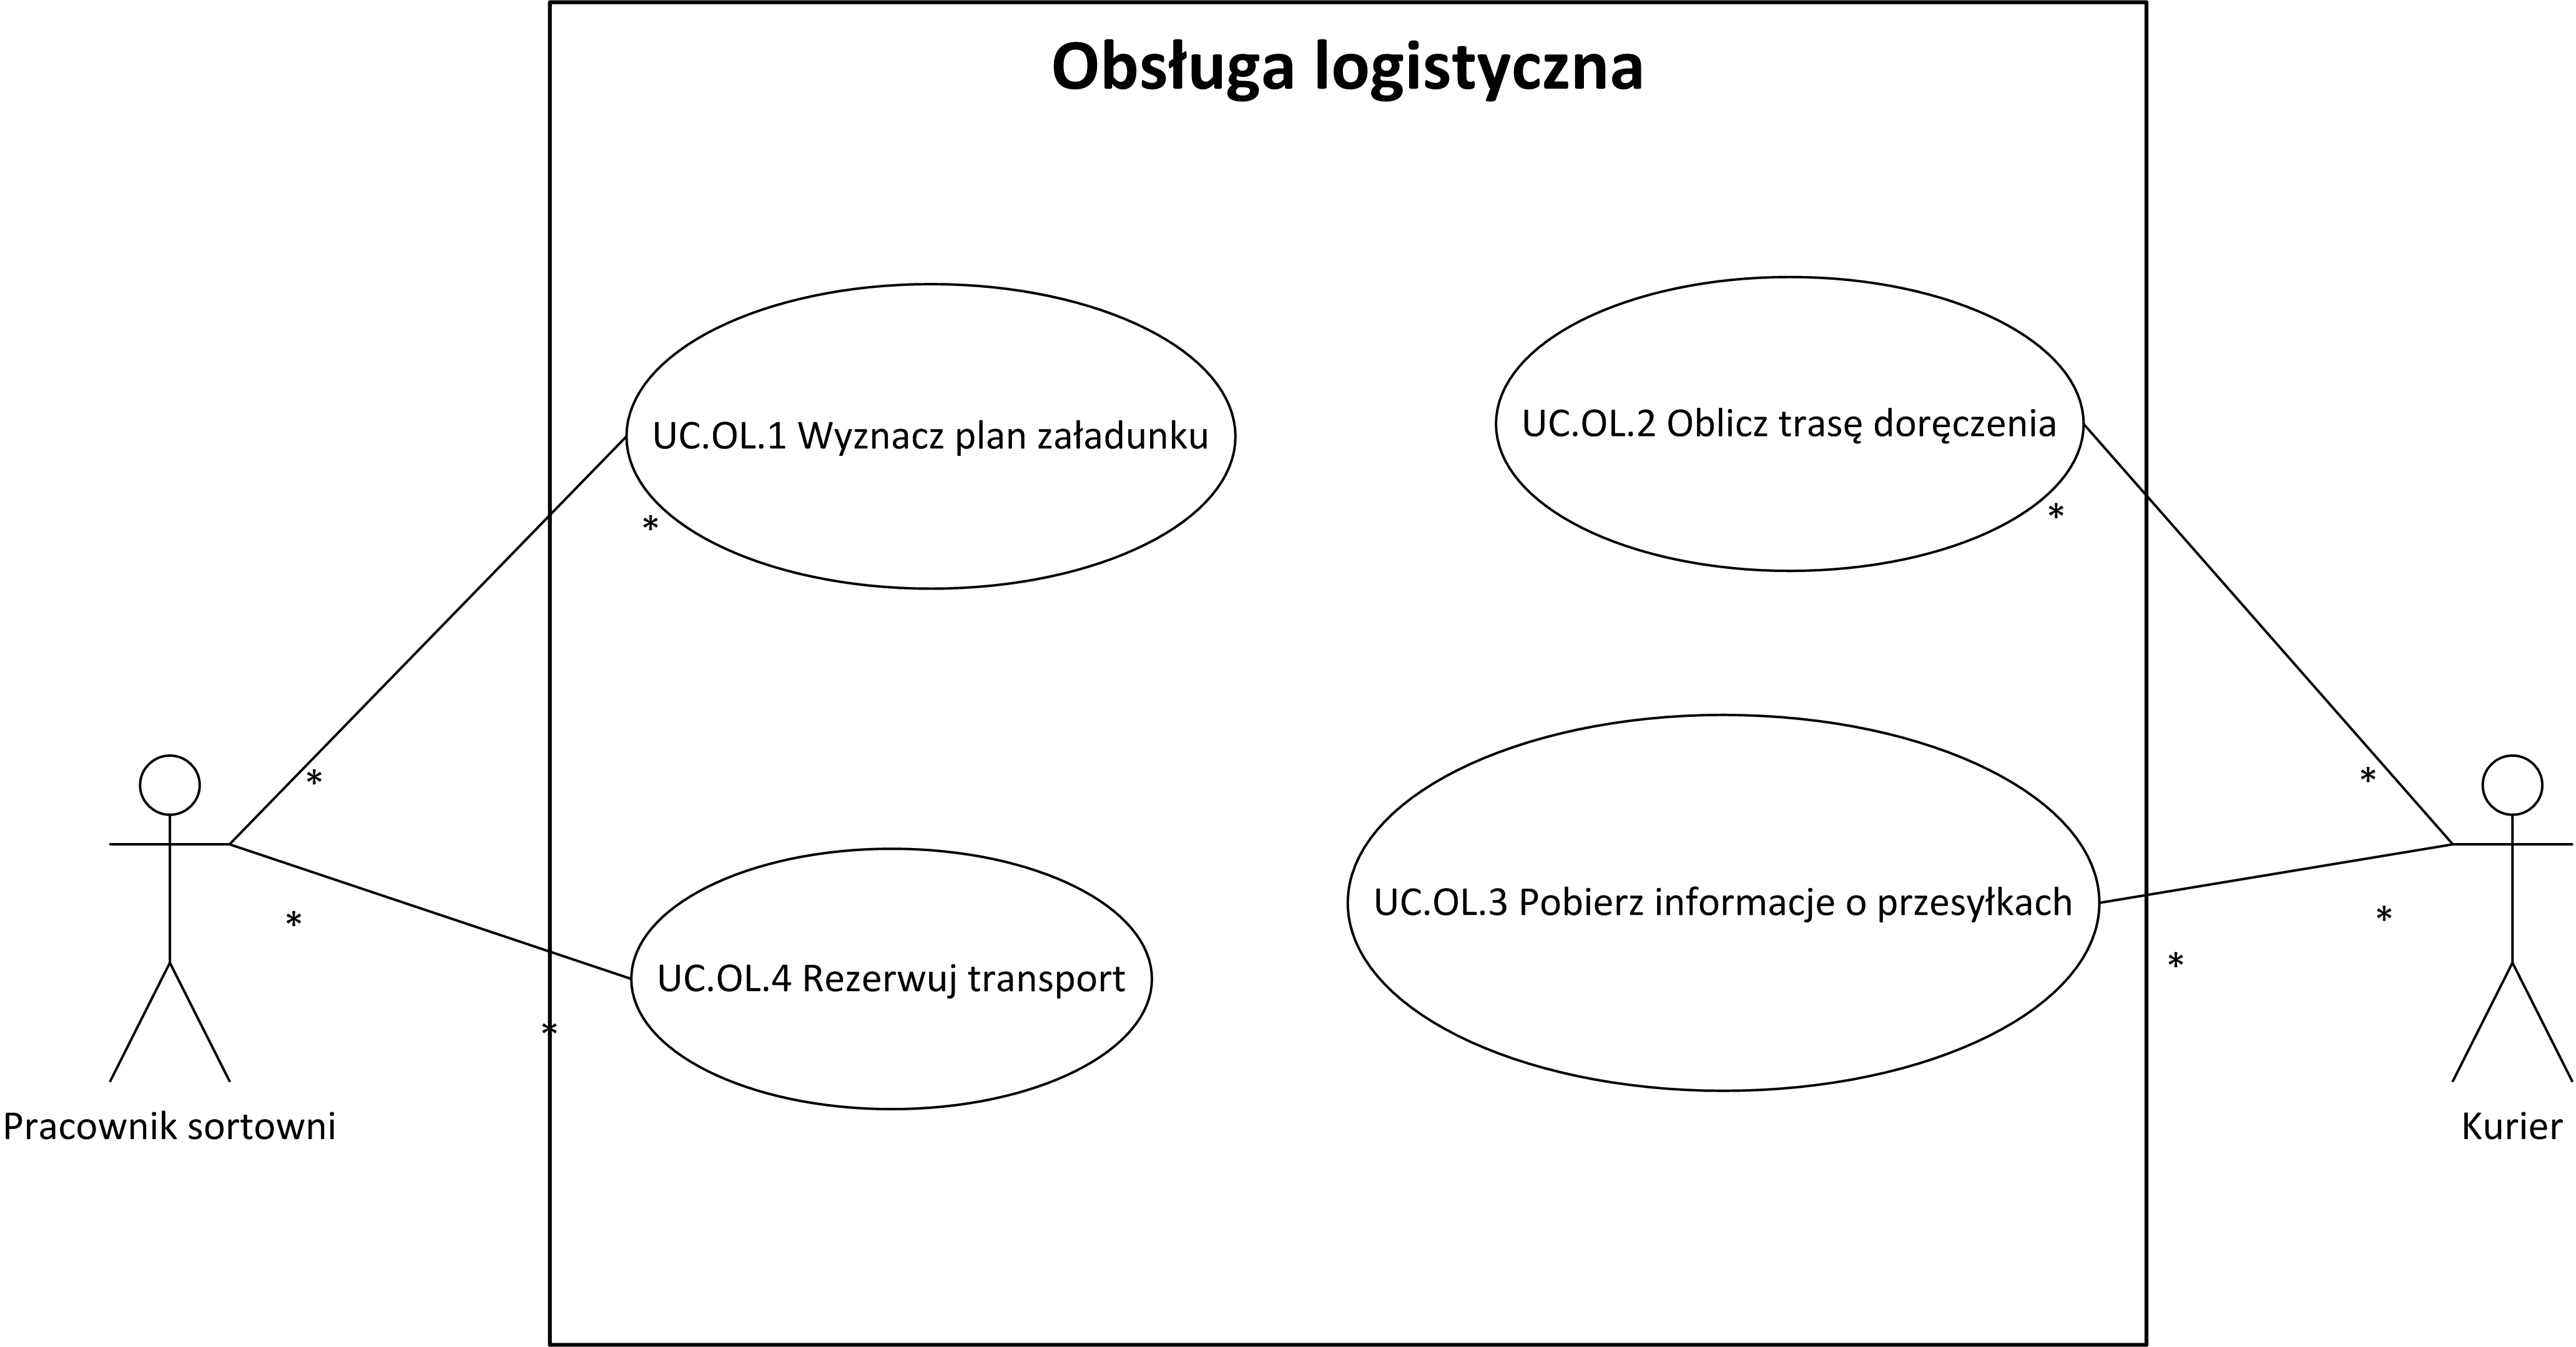
\includegraphics[width=\textwidth]{img/obs_log_uc}
\end{figure}

\subsubsection*{Scenariusze przypadków użycia}
\begin{center}
\begin{longtable}[h]{|p{1.6cm}|p{13.5cm}|}
\hline
\textbf{ID:} & UC.OL.1 \\ \hline
\textbf{Nazwa:} & Wyznacz plan załadunku \\ \hline
\multicolumn{2}{|p{15.1cm}|}{\textbf{Aktorzy główni:} Pracownik sortowni} \\
\multicolumn{2}{|p{15.1cm}|}{\textbf{Aktorzy pomocniczy:} \textit{brak}} \\
\multicolumn{2}{|p{15.1cm}|}{\textbf{Poziom:} Użytkownika} \\
\multicolumn{2}{|p{15.1cm}|}{\textbf{Priorytet:} Wysoki} \\
\hline
\multicolumn{2}{|p{15.1cm}|}{\textbf{Opis:}} \\
\multicolumn{2}{|p{15.1cm}|}{
Pracownik sortowni chce uzyskać plan załadunku przesyłek, które oczekują na doręczenie.
} \\ \hline
\multicolumn{2}{|p{15.1cm}|}{\textbf{Wyzwalacze:}} \\
\multicolumn{2}{|p{15.1cm}|}{
Wybranie odpowiedniej opcji w aplikacji klienckiej.
} \\ \hline
\multicolumn{2}{|p{15.1cm}|}{\textbf{Warunki początkowe:}} \\
\multicolumn{2}{|p{15.1cm}|}{
Aktor musi być zalogowany do SWPFK.
} \\ \hline
\multicolumn{2}{|p{15.1cm}|}{\textbf{Warunki końcowe:}} \\
\multicolumn{2}{|p{15.1cm}|}{
System wyświetla przygotowany plan załadunku przesyłek.
} \\ \hline
\multicolumn{2}{|p{15.1cm}|}{\textbf{Scenariusz główny:}} \\
\multicolumn{2}{|p{15.1cm}|}{
\begin{enumerate}
\item Aktor wybiera opcję ''Oblicz plan załadunku''.
\item System wyświetla listę przesyłek, które oczekują na doręczenie. Domyślnie wszystkie przesyłki są zaznaczone.
\item Aktor odznacza przesyłki, które chce wyłączyć z doręczenia.
\item Aktor wyzwala przeliczanie wybierając funkcję ''Wyznacz plan''.
\item System gromadzi parametry wybranych przesyłek.
\item System pobiera informacje o pojazdach dostępnych do doręczenia.
\item System wyznacza plan załadunku uwzględniając pobrane informacje oraz możliwe trasy doręczeń.
\item System prezentuje plan w tabelach reprezentujących pojazdy, które zawierają wyszczególnione przesyłki w kolejności jakiej powinny być załadowane do pojazdu.
\end{enumerate}
} \\ \hline
\multicolumn{2}{|p{15.1cm}|}{\textbf{Scenariusze alternatywne i rozszerzenia:}} \\
\multicolumn{2}{|p{15.1cm}|}{
3.a Aktor odznaczył wszystkie możliwe przesyłki. \newline
3.a.1 System prezentuje ostrzeżenie, że nie wybrano żadnej przesyłki. \newline
3.a.2 Aktor zaznacza wybrane przesyłki. \newline
3.a.3 Powrót do punktu 4 scenariusza głównego. \newline
\newline
7.a Wyznaczenie planu załadunku nie powiodło. \newline
7.a.1 System prezentuje informacje o błędzie podczas wyznaczania planu. \newline
7.a.2 Aktor koryguje listę przesyłek do doręczenia. \newline
7.a.3 Powrót do punktu 4 scenariusza głównego.
} \\ \hline
\multicolumn{2}{|p{15.1cm}|}{\textbf{Wyjątki:}} \\
\multicolumn{2}{|p{15.1cm}|}{
System posiada nieaktualne informacje o pojazdach, co powoduje wyznaczenie błędnego planu.
} \\ \hline
\multicolumn{2}{|p{15.1cm}|}{\textbf{Dodatkowe wymagania:}} \\
\multicolumn{2}{|p{15.1cm}|}{
\textit{brak}
} \\
\hline
\end{longtable}
\end{center}

\begin{center}
\begin{longtable}[h]{|p{1.6cm}|p{13.5cm}|}
\hline
\textbf{ID:} & UC.OL.2 \\ \hline
\textbf{Nazwa:} & Oblicz trasę doręczenia \\ \hline
\multicolumn{2}{|p{15.1cm}|}{\textbf{Aktorzy główni:} Kurier} \\
\multicolumn{2}{|p{15.1cm}|}{\textbf{Aktorzy pomocniczy:} \textit{brak}} \\
\multicolumn{2}{|p{15.1cm}|}{\textbf{Poziom:} Użytkownika} \\
\multicolumn{2}{|p{15.1cm}|}{\textbf{Priorytet:} Wysoki} \\
\hline
\multicolumn{2}{|p{15.1cm}|}{\textbf{Opis:}} \\
\multicolumn{2}{|p{15.1cm}|}{
Kurier chce wygenerować trasę doręczenia przesyłek.
} \\ \hline
\multicolumn{2}{|p{15.1cm}|}{\textbf{Wyzwalacze:}} \\
\multicolumn{2}{|p{15.1cm}|}{
Aktor wybiera opcję ''Wyznacz trasę doręczenia'' w aplikacji mobilnej.
} \\ \hline
\multicolumn{2}{|p{15.1cm}|}{\textbf{Warunki początkowe:}} \\
\multicolumn{2}{|p{15.1cm}|}{
1. Został wygenerowany plan załadunku pojazdów. \newline
2. Kurier wprowadził numer pojazdu do aplikacji mobilnej.
} \\ \hline
\multicolumn{2}{|p{15.1cm}|}{\textbf{Warunki końcowe:}} \\
\multicolumn{2}{|p{15.1cm}|}{
System prezentuje obliczoną trasę doręczenia.
} \\ \hline
\multicolumn{2}{|p{15.1cm}|}{\textbf{Scenariusz główny:}} \\
\multicolumn{2}{|p{15.1cm}|}{
\begin{enumerate}
\item Aktor wybiera opcję ''Wyznacz trasę doręczenia''.
\item Aplikacja mobilna przesyła żądanie do modułu serwerowego o obliczenie trasy doręczenia.
\item Moduł serwerowy wyznacza trasę na podstawie informacji o przesyłkach znajdujących się w pojeździe.
\item Moduł serwerowy przesyła wyznaczoną trasę do aplikacji klienckiej.
\item Aplikacja mobilna prezentuje trasę doręczenia.
\item Aktor wybiera opcję ''Zapisz trasę''.
\item Aplikacja mobilna zapisuje wyznaczoną trasę.
\end{enumerate}
} \\ \hline
\multicolumn{2}{|p{15.1cm}|}{\textbf{Scenariusze alternatywne i rozszerzenia:}} \\
\multicolumn{2}{|p{15.1cm}|}{
3.a Wystąpił błąd podczas obliczania trasy. \newline
3.a.1 Moduł serwerowy przesyła informacje o zaistniałym błędzie. \newline
3.a.2 Aplikacja mobilna prezentuje informacje o błędzie. \newline
3.a.3 Przypadek użycia kończy się.
} \\ \hline
\multicolumn{2}{|p{15.1cm}|}{\textbf{Wyjątki:}} \\
\multicolumn{2}{|p{15.1cm}|}{
Terminal mobilny nie ma połączenia z modułem serwerowym.
} \\ \hline
\multicolumn{2}{|p{15.1cm}|}{\textbf{Dodatkowe wymagania:}} \\
\multicolumn{2}{|p{15.1cm}|}{
\textit{brak}
} \\
\hline
\end{longtable}
\end{center}

\begin{center}
\begin{longtable}[h]{|p{1.6cm}|p{13.5cm}|}
\hline
\textbf{ID:} & UC.OL.3 \\ \hline
\textbf{Nazwa:} & Pobierz informacje o przesyłkach \\ \hline
\multicolumn{2}{|p{15.1cm}|}{\textbf{Aktorzy główni:} Kurier} \\
\multicolumn{2}{|p{15.1cm}|}{\textbf{Aktorzy pomocniczy:} \textit{brak}} \\
\multicolumn{2}{|p{15.1cm}|}{\textbf{Poziom:} Użytkownika} \\
\multicolumn{2}{|p{15.1cm}|}{\textbf{Priorytet:} Średni} \\
\hline
\multicolumn{2}{|p{15.1cm}|}{\textbf{Opis:}} \\
\multicolumn{2}{|p{15.1cm}|}{
Kurier chce pobrać na terminal mobilny informacje o przesyłkach, które ma doręczyć.
} \\ \hline
\multicolumn{2}{|p{15.1cm}|}{\textbf{Wyzwalacze:}} \\
\multicolumn{2}{|p{15.1cm}|}{
Aktor wybiera opcję ''Pobierz informacje o przesyłkach''.
} \\ \hline
\multicolumn{2}{|p{15.1cm}|}{\textbf{Warunki początkowe:}} \\
\multicolumn{2}{|p{15.1cm}|}{
Został wygenerowany plan załadunku pojazdów.
} \\ \hline
\multicolumn{2}{|p{15.1cm}|}{\textbf{Warunki końcowe:}} \\
\multicolumn{2}{|p{15.1cm}|}{
Informacje o przesyłkach zostają zapisane na terminalu mobilnym.
} \\ \hline
\multicolumn{2}{|p{15.1cm}|}{\textbf{Scenariusz główny:}} \\
\multicolumn{2}{|p{15.1cm}|}{
\begin{enumerate}
\item Aktor wybiera opcję ''Pobierz informacje o przesyłkach''.
\item Aplikacja mobilna przesyła żądanie do modułu serwerowego.
\item Moduł serwerowy pobiera informacje o przesyłkach i przesyła je do aplikacji mobilnej.
\item Aplikacja mobilna zapisuje otrzymane informacje.
\item Aplikacja mobilna prezentuje otrzymane dane.
\end{enumerate}
} \\ \hline
\multicolumn{2}{|p{15.1cm}|}{\textbf{Scenariusze alternatywne i rozszerzenia:}} \\
\multicolumn{2}{|p{15.1cm}|}{
\textit{brak}
} \\ \hline
\multicolumn{2}{|p{15.1cm}|}{\textbf{Wyjątki:}} \\
\multicolumn{2}{|p{15.1cm}|}{
Terminal mobilny nie ma połączenia z modułem serwerowym.
} \\ \hline
\multicolumn{2}{|p{15.1cm}|}{\textbf{Dodatkowe wymagania:}} \\
\multicolumn{2}{|p{15.1cm}|}{
\textit{brak}
} \\
\hline
\end{longtable}
\end{center}

\begin{center}
\begin{longtable}[h]{|p{1.6cm}|p{13.5cm}|}
\hline
\textbf{ID:} & UC.OL.4 \\ \hline
\textbf{Nazwa:} & Rezerwuj transport \\ \hline
\multicolumn{2}{|p{15.1cm}|}{\textbf{Aktorzy główni:} Pracownik sortowni} \\
\multicolumn{2}{|p{15.1cm}|}{\textbf{Aktorzy pomocniczy:} 
Zewnętrzna firma transportowa} \\
\multicolumn{2}{|p{15.1cm}|}{\textbf{Poziom:} Użytkownika} \\
\multicolumn{2}{|p{15.1cm}|}{\textbf{Priorytet:} Wysoki} \\
\hline
\multicolumn{2}{|p{15.1cm}|}{\textbf{Opis:}} \\
\multicolumn{2}{|p{15.1cm}|}{
Pracownik sortowni chce zarezerwować transport w celu przewiezienia oczekujących przesyłek.
} \\ \hline
\multicolumn{2}{|p{15.1cm}|}{\textbf{Wyzwalacze:}} \\
\multicolumn{2}{|p{15.1cm}|}{
Aktor wybiera opcję ''Rezerwuj transport'' w aplikacji klienckiej.
} \\ \hline
\multicolumn{2}{|p{15.1cm}|}{\textbf{Warunki początkowe:}} \\
\multicolumn{2}{|p{15.1cm}|}{
\textit{brak}
} \\ \hline
\multicolumn{2}{|p{15.1cm}|}{\textbf{Warunki końcowe:}} \\
\multicolumn{2}{|p{15.1cm}|}{
Transport dla wyznaczonych przesyłek zostaje zarezerwowany we flocie Firmy Kurierskiej lub flocie firmy zewnętrznej.
} \\ \hline
\multicolumn{2}{|p{15.1cm}|}{\textbf{Scenariusz główny:}} \\
\multicolumn{2}{|p{15.1cm}|}{
\begin{enumerate}
\item Aktor wybiera opcję ''Rezerwuj transport'' w aplikacji klienckiej.
\item Aplikacja kliencka prezentuje listę przesyłek oczekujących na przesłanie do innych sortowni. Domyślnie wszystkie przesyłki są zaznaczone.
\item Aktor odznacza przesyłki, które nie mają zostać przesłane.
\item Aplikacja kliencka przesyła żądanie rezerwacji do modułu serwerowego.
\item Moduł serwerowy wyznacza sieć połączeń na jakich trzeba przetransportować wybrane przesyłki.
\item Moduł serwerowy pobiera informacje o dostępnej flocie wewnętrznej.
\item Moduł serwerowy komunikuje się z systemami zewnętrznych firm transportowych w celu pobrania informacji o dostępnej flocie.
\item Moduł serwerowy wyznacza listę pojazdów jakie należy zarezerwować i przesyła ją do aplikacji klienckiej.
\item Aplikacja kliencka prezentuje wyznaczony plan przewozu.
\item Aktor zatwierdza wyznaczony plan.
\item Moduł serwerowy rezerwuje pojazdy we flocie wewnętrznej oraz przesyła żądania rezerwacji do zewnętrznych firm.
\item Moduł serwerowy generuje potwierdzenie pomyślnej rezerwacji pojazdów oraz przesyła je do aplikacji klienckiej.
\item Aplikacja kliencka prezentuje potwierdzenie rezerwacji.
\end{enumerate}
} \\ \hline
\multicolumn{2}{|p{15.1cm}|}{\textbf{Scenariusze alternatywne i rozszerzenia:}} \\
\multicolumn{2}{|p{15.1cm}|}{
8.a Wyznaczenie listy pojazdów jest niemożliwe z powodu braku ich dostępności. \newline
8.a.1 Moduł serwerowy generuje ostrzeżenie i przesyła je do aplikacji klienckiej. \newline
8.a.2 Aplikacja kliencka prezentuje informacje o niepowodzeniu. \newline
8.a.3 Przypadek użycia kończy się.\newline
\newline
11.a Rezerwacja pojazdów została odrzucona. \newline
11.a.1 Moduł serwerowy przesyła powód odrzucenia do aplikacji klienckiej.\newline
11.a.2 Aplikacja kliencka prezentuje informacje o niepowodzeniu. \newline
11.a.3 Aktor wybiera opcję ''Spróbuj ponownie''. \newline
11.a.4 Powrót do punktu 4 scenariusza głównego.
} \\ \hline
\multicolumn{2}{|p{15.1cm}|}{\textbf{Wyjątki:}} \\
\multicolumn{2}{|p{15.1cm}|}{
Aplikacja kliencka nie ma połączenia z modułem serwerowym.
} \\ \hline
\multicolumn{2}{|p{15.1cm}|}{\textbf{Dodatkowe wymagania:}} \\
\multicolumn{2}{|p{15.1cm}|}{
\textit{brak}
} \\
\hline
\end{longtable}
\end{center}

\subsection{Obsługa finansowa}
\subsubsection*{Opis}
Moduł zawiera funkcjonalności z zakresu obsługi finansowej klientów biznesowych oraz z zakresu windykacji.

\subsubsection*{Przypadki użycia}
\begin{figure}[H]
\centering
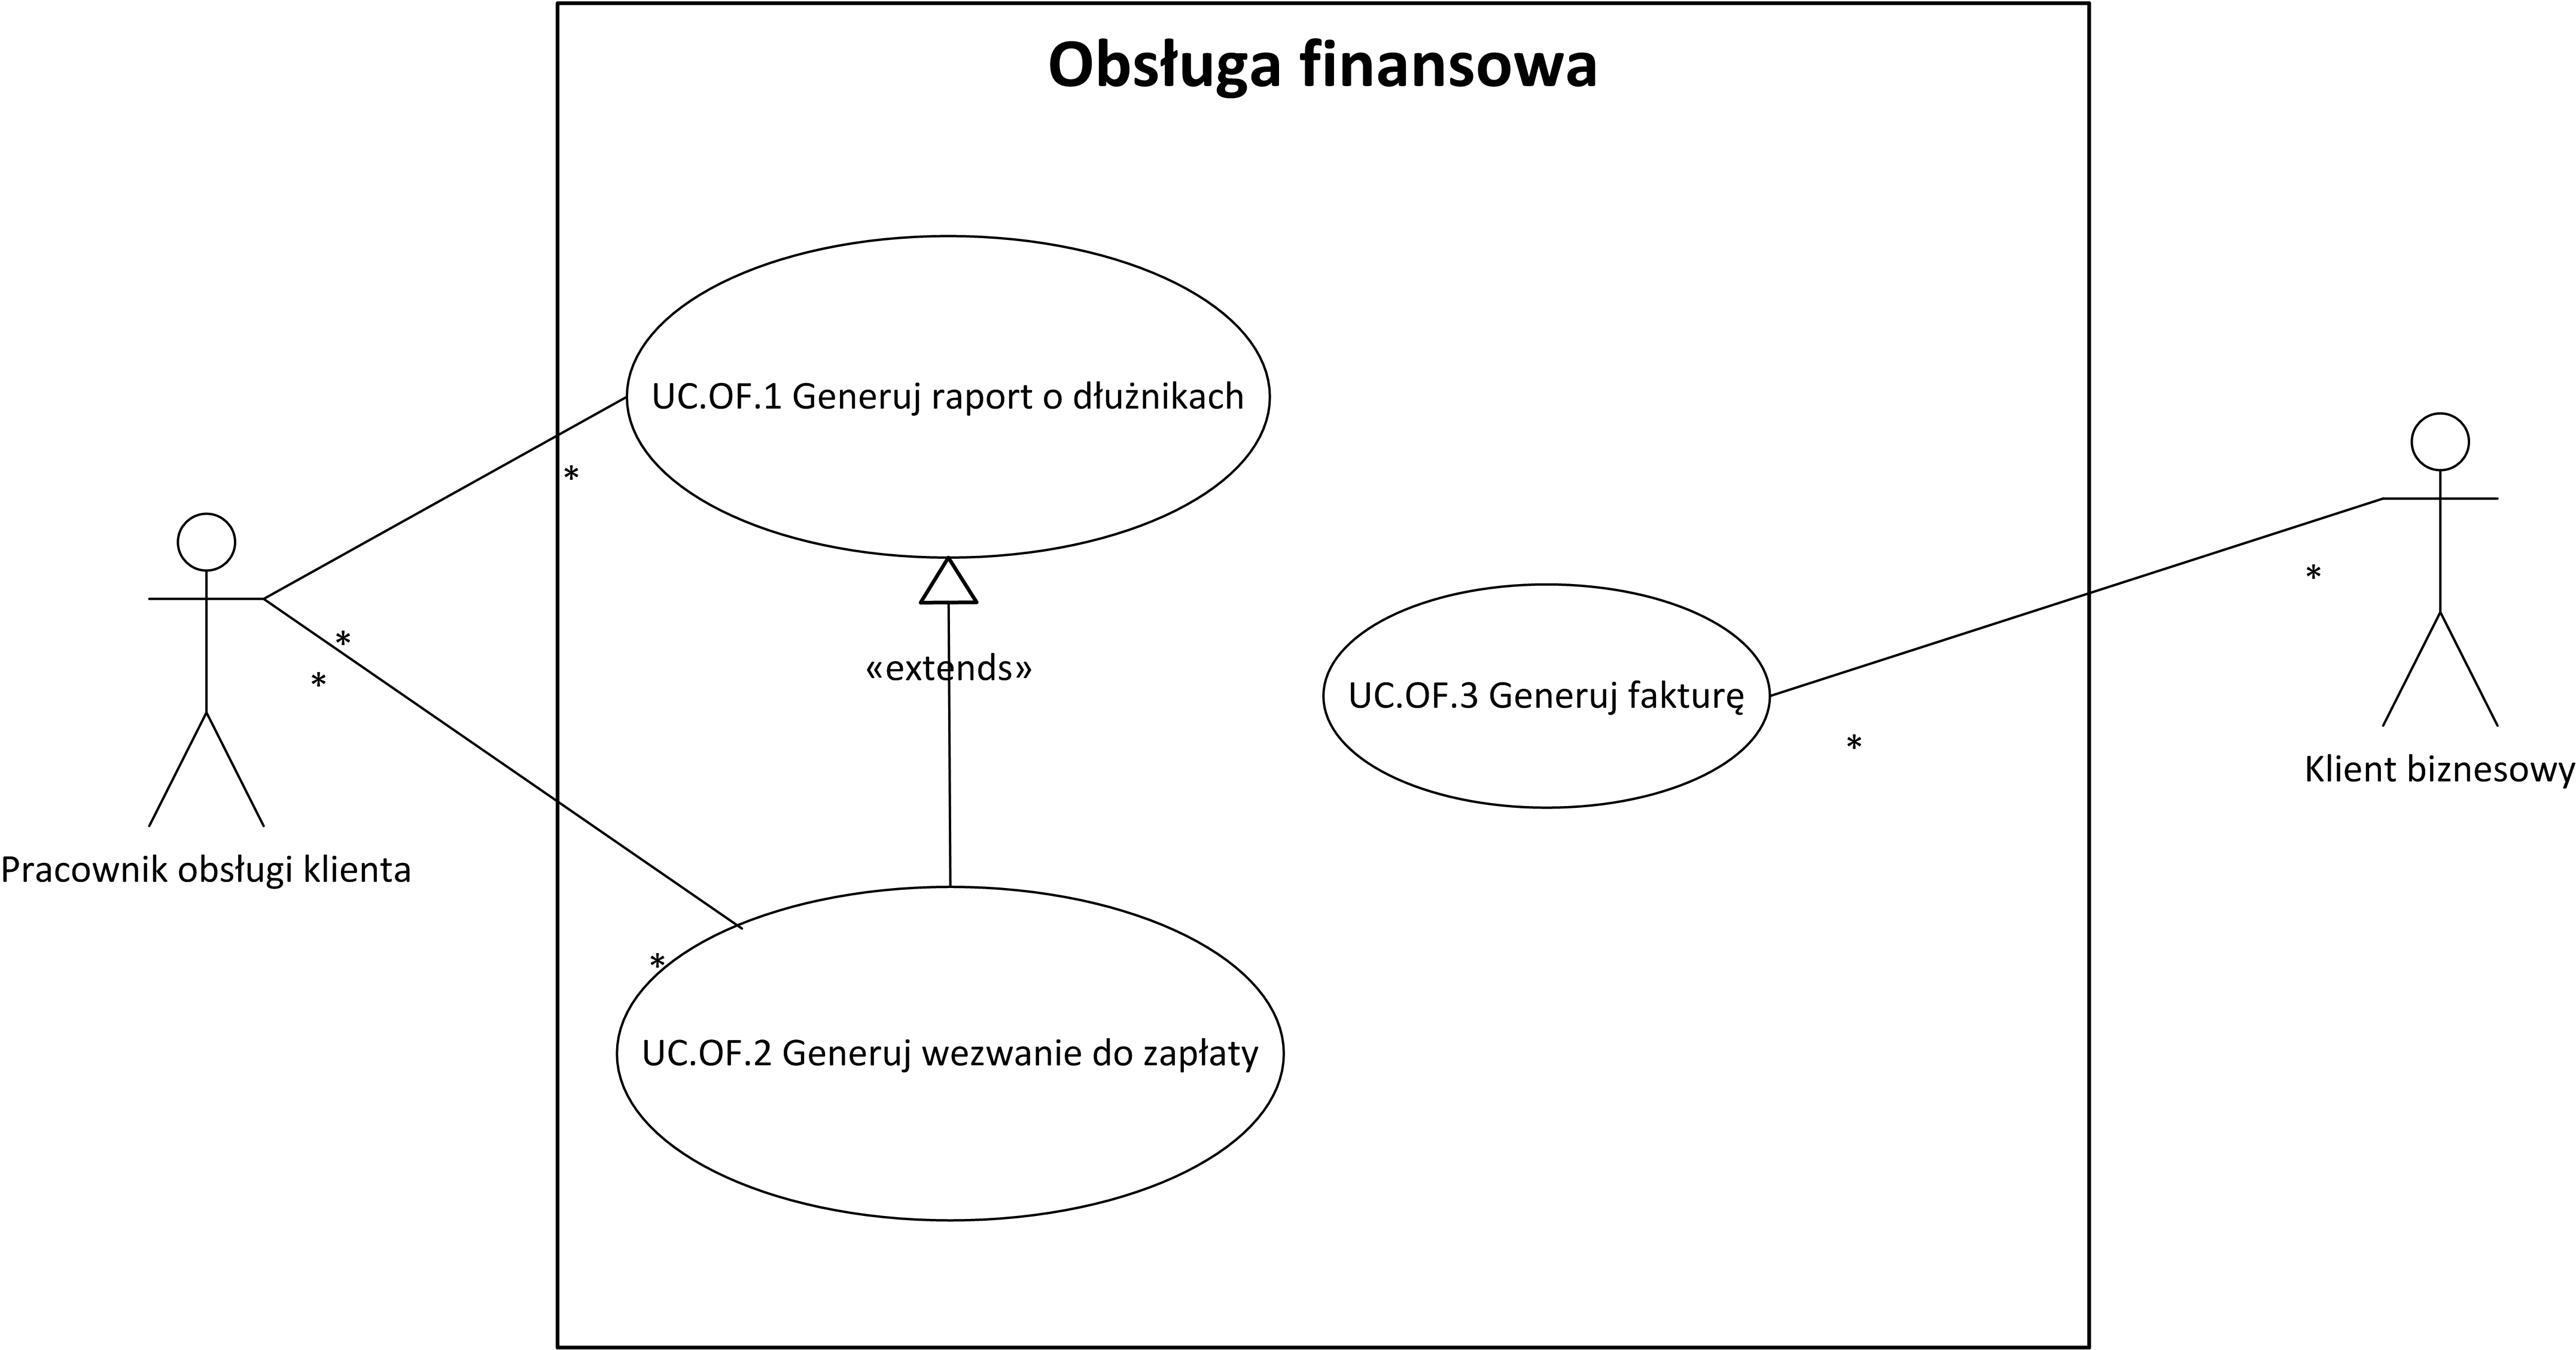
\includegraphics[width=\textwidth]{img/obs_fin_uc}
\end{figure}

\subsubsection*{Scenariusze przypadków użycia}
\begin{center}
\begin{longtable}[h]{|p{1.6cm}|p{13.5cm}|}
\hline
\textbf{ID:} & UC.OF.1 \\ \hline
\textbf{Nazwa:} & Generuj raport o dłużnikach \\ \hline
\multicolumn{2}{|p{15.1cm}|}{\textbf{Aktorzy główni:} Pracownik obsługi klienta} \\
\multicolumn{2}{|p{15.1cm}|}{\textbf{Aktorzy pomocniczy:} 
\textit{brak}} \\
\multicolumn{2}{|p{15.1cm}|}{\textbf{Poziom:} Użytkownika} \\
\multicolumn{2}{|p{15.1cm}|}{\textbf{Priorytet:} Średni} \\
\hline
\multicolumn{2}{|p{15.1cm}|}{\textbf{Opis:}} \\
\multicolumn{2}{|p{15.1cm}|}{
Pracownik chce wygenerować raport o klient zalegających z płatnościami za usługi.
} \\ \hline
\multicolumn{2}{|p{15.1cm}|}{\textbf{Wyzwalacze:}} \\
\multicolumn{2}{|p{15.1cm}|}{
Aktor wybiera opcję ''Generuj raport o dłużnikach'' w aplikacji klienckiej.
} \\ \hline
\multicolumn{2}{|p{15.1cm}|}{\textbf{Warunki początkowe:}} \\
\multicolumn{2}{|p{15.1cm}|}{
Aktor jest zalogowany w aplikacji klienckiej.
} \\ \hline
\multicolumn{2}{|p{15.1cm}|}{\textbf{Warunki końcowe:}} \\
\multicolumn{2}{|p{15.1cm}|}{
Raport o dłużnikach zostaje zaprezentowany aktorowi.
} \\ \hline
\multicolumn{2}{|p{15.1cm}|}{\textbf{Scenariusz główny:}} \\
\multicolumn{2}{|p{15.1cm}|}{
\begin{enumerate}
\item Aktor wybiera opcję ''Generuj raport o dłużnikach'' w aplikacji klienckiej.
\item System pobiera listę dostępnych klientów biznesowych.
\item System prezentuje listę klientów biznesowych.
\item Aktor zaznacza klientów o których chce sporządzić raport.
\item System generuje raporty zadłużenia dla zaznaczonych klientów.
\item System zapisuje raporty w aplikacji.
\item System umożliwia otwarcie wygenerowanych raportów.
\end{enumerate}
} \\ \hline
\multicolumn{2}{|p{15.1cm}|}{\textbf{Scenariusze alternatywne i rozszerzenia:}} \\
\multicolumn{2}{|p{15.1cm}|}{
4.a Aktor nie wybrał żadnego klienta. \newline
4.a.1 System prezentuje ostrzeżenie o nie wybraniu żadnego klienta. \newline
4.a.2 Aktor koryguje listę wybranych klientów. \newline
4.a.3 Powrót do punktu 5 scenariusza głównego.
} \\ \hline
\multicolumn{2}{|p{15.1cm}|}{\textbf{Wyjątki:}} \\
\multicolumn{2}{|p{15.1cm}|}{
\textit{brak}
} \\ \hline
\multicolumn{2}{|p{15.1cm}|}{\textbf{Dodatkowe wymagania:}} \\
\multicolumn{2}{|p{15.1cm}|}{
\textit{brak}
} \\
\hline
\end{longtable}
\end{center}

\begin{center}
\begin{longtable}[h]{|p{1.6cm}|p{13.5cm}|}
\hline
\textbf{ID:} & UC.OF.2 \\ \hline
\textbf{Nazwa:} & Generuj wezwanie do zapłaty \\ \hline
\multicolumn{2}{|p{15.1cm}|}{\textbf{Aktorzy główni:} Pracownik obsługi klienta} \\
\multicolumn{2}{|p{15.1cm}|}{\textbf{Aktorzy pomocniczy:} 
\textit{brak}} \\
\multicolumn{2}{|p{15.1cm}|}{\textbf{Poziom:} Użytkownika} \\
\multicolumn{2}{|p{15.1cm}|}{\textbf{Priorytet:} Średni} \\
\hline
\multicolumn{2}{|p{15.1cm}|}{\textbf{Opis:}} \\
\multicolumn{2}{|p{15.1cm}|}{
Aktor chce wygenerować wezwanie do zapłaty dla klienta biznesowego, który zalega z płatnościami za usługi.
} \\ \hline
\multicolumn{2}{|p{15.1cm}|}{\textbf{Wyzwalacze:}} \\
\multicolumn{2}{|p{15.1cm}|}{
Aktor wygenerował Raporty o zadłużeniach i wybrał opcję ''Utwórz wezwanie do zapłaty'' obok jednego z raportów.
} \\ \hline
\multicolumn{2}{|p{15.1cm}|}{\textbf{Warunki początkowe:}} \\
\multicolumn{2}{|p{15.1cm}|}{
1. Aktor jest zalogowany do aplikacji klienckiej. \newline
2. Aktor wygenerował listę raportów o zadłużeniach.
} \\ \hline
\multicolumn{2}{|p{15.1cm}|}{\textbf{Warunki końcowe:}} \\
\multicolumn{2}{|p{15.1cm}|}{
Wezwanie do zapłaty zostaje wygenerowane i system umożliwia jego wydruk.
} \\ \hline
\multicolumn{2}{|p{15.1cm}|}{\textbf{Scenariusz główny:}} \\
\multicolumn{2}{|p{15.1cm}|}{
\begin{enumerate}
\item Aktor wybiera opcję ''Utwórz wezwanie do zapłaty'' obok jednego z raportów o zadłużeniach.
\item System prezentuje listę pozycji które składają się na raport.
\item Aktor wybiera pozycje dla których chce wygenerować wezwanie.
\item System generuje wezwanie do zapłaty dla wskazanego klienta biznesowego oraz wybranych pozycji.
\item System prezentuje wygenerowane wezwanie do zapłaty.
\item Aktor wybiera opcję ''Drukuj raport'' w celu wydrukowania raportu.
\item System przesyła żądanie wydruku do drukarki.
\end{enumerate}
} \\ \hline
\multicolumn{2}{|p{15.1cm}|}{\textbf{Scenariusze alternatywne i rozszerzenia:}} \\
\multicolumn{2}{|p{15.1cm}|}{
3.a Aktor nie wybrał żadnej pozycji zadłużenia. \newline
3.a.1 System prezentuje ostrzeżenie. \newline
3.a.2 Aktor poprawia wybór pozycji. \newline
3.a.3 Powrót do punktu 4 scenariusza głównego. \newline
\newline
6.a Aplikacja kliencka nie ma połączenia z drukarką. \newline
6.a.1 System blokuje przycisk ''Drukuj raport''. \newline
6.a.2 Przypadek użycia kończy się. \newline
} \\ \hline
\multicolumn{2}{|p{15.1cm}|}{\textbf{Wyjątki:}} \\
\multicolumn{2}{|p{15.1cm}|}{
\textit{brak}} \\ \hline
\multicolumn{2}{|p{15.1cm}|}{\textbf{Dodatkowe wymagania:}} \\
\multicolumn{2}{|p{15.1cm}|}{
Dostęp aplikacji klienckiej do drukarki.
} \\
\hline
\end{longtable}
\end{center}

\begin{center}
\begin{longtable}[h]{|p{1.6cm}|p{13.5cm}|}
\hline
\textbf{ID:} & UC.OF.3 \\ \hline
\textbf{Nazwa:} & Generuj fakturę \\ \hline
\multicolumn{2}{|p{15.1cm}|}{\textbf{Aktorzy główni:} Klient biznesowy} \\
\multicolumn{2}{|p{15.1cm}|}{\textbf{Aktorzy pomocniczy:} 
\textit{brak}} \\
\multicolumn{2}{|p{15.1cm}|}{\textbf{Poziom:} Użytkownika} \\
\multicolumn{2}{|p{15.1cm}|}{\textbf{Priorytet:} Wysoki} \\
\hline
\multicolumn{2}{|p{15.1cm}|}{\textbf{Opis:}} \\
\multicolumn{2}{|p{15.1cm}|}{
Klient biznesowy chce wygenerować fakturę za wybrane usługi.
} \\ \hline
\multicolumn{2}{|p{15.1cm}|}{\textbf{Wyzwalacze:}} \\
\multicolumn{2}{|p{15.1cm}|}{
Aktor wybiera opcję ''Generuj fakturę'' w interfejsie internetowym.
} \\ \hline
\multicolumn{2}{|p{15.1cm}|}{\textbf{Warunki początkowe:}} \\
\multicolumn{2}{|p{15.1cm}|}{
Aktor jest zalogowany w interfejsie internetowym.
} \\ \hline
\multicolumn{2}{|p{15.1cm}|}{\textbf{Warunki końcowe:}} \\
\multicolumn{2}{|p{15.1cm}|}{
Faktura zostaje wygenerowana i system umożliwia pobrania jej w formacie PDF.
} \\ \hline
\multicolumn{2}{|p{15.1cm}|}{\textbf{Scenariusz główny:}} \\
\multicolumn{2}{|p{15.1cm}|}{
\begin{enumerate}
\item Aktor wybiera opcję ''Generuj fakturę''.
\item System prezentuje listę nieopłaconych usług klienta.
\item Aktor wybiera usługi za które chce uzyskać fakturę.
\item System generuje fakturę na podstawie wskazanych pozycji.
\item System prezentuje wygenerowaną fakturę.
\item System umożliwia pobranie faktury w formie pliku PDF.
\end{enumerate}
} \\ \hline
\multicolumn{2}{|p{15.1cm}|}{\textbf{Scenariusze alternatywne i rozszerzenia:}} \\
\multicolumn{2}{|p{15.1cm}|}{
3.a Aktor nie wskazał żadnej pozycji. \newline
3.a.1 System prezentuje ostrzeżenie. \newline
3.a.2 Aktor koryguje swój wybór. \newline
3.a.3 Powrót do punktu 4 scenariusza głównego. 
} \\ \hline
\multicolumn{2}{|p{15.1cm}|}{\textbf{Wyjątki:}} \\
\multicolumn{2}{|p{15.1cm}|}{
\textit{brak}
} \\ \hline
\multicolumn{2}{|p{15.1cm}|}{\textbf{Dodatkowe wymagania:}} \\
\multicolumn{2}{|p{15.1cm}|}{
\textit{brak}
} \\
\hline
\end{longtable}
\end{center}

\subsection{Moduł informacyjny i obsługi klienta}
\subsubsection*{Opis}
Moduł zawiera funkcjonalności dostarczające informację klientowi informację o usługach Firmy Kurierskiej. Zawiera również opis funkcjonalności logowania do systemu oraz obsługę reklamacji. Definiuje także funkcję nadania przesyłki w POK.

\subsubsection*{Przypadki użycia}
\begin{figure}[H]
\centering
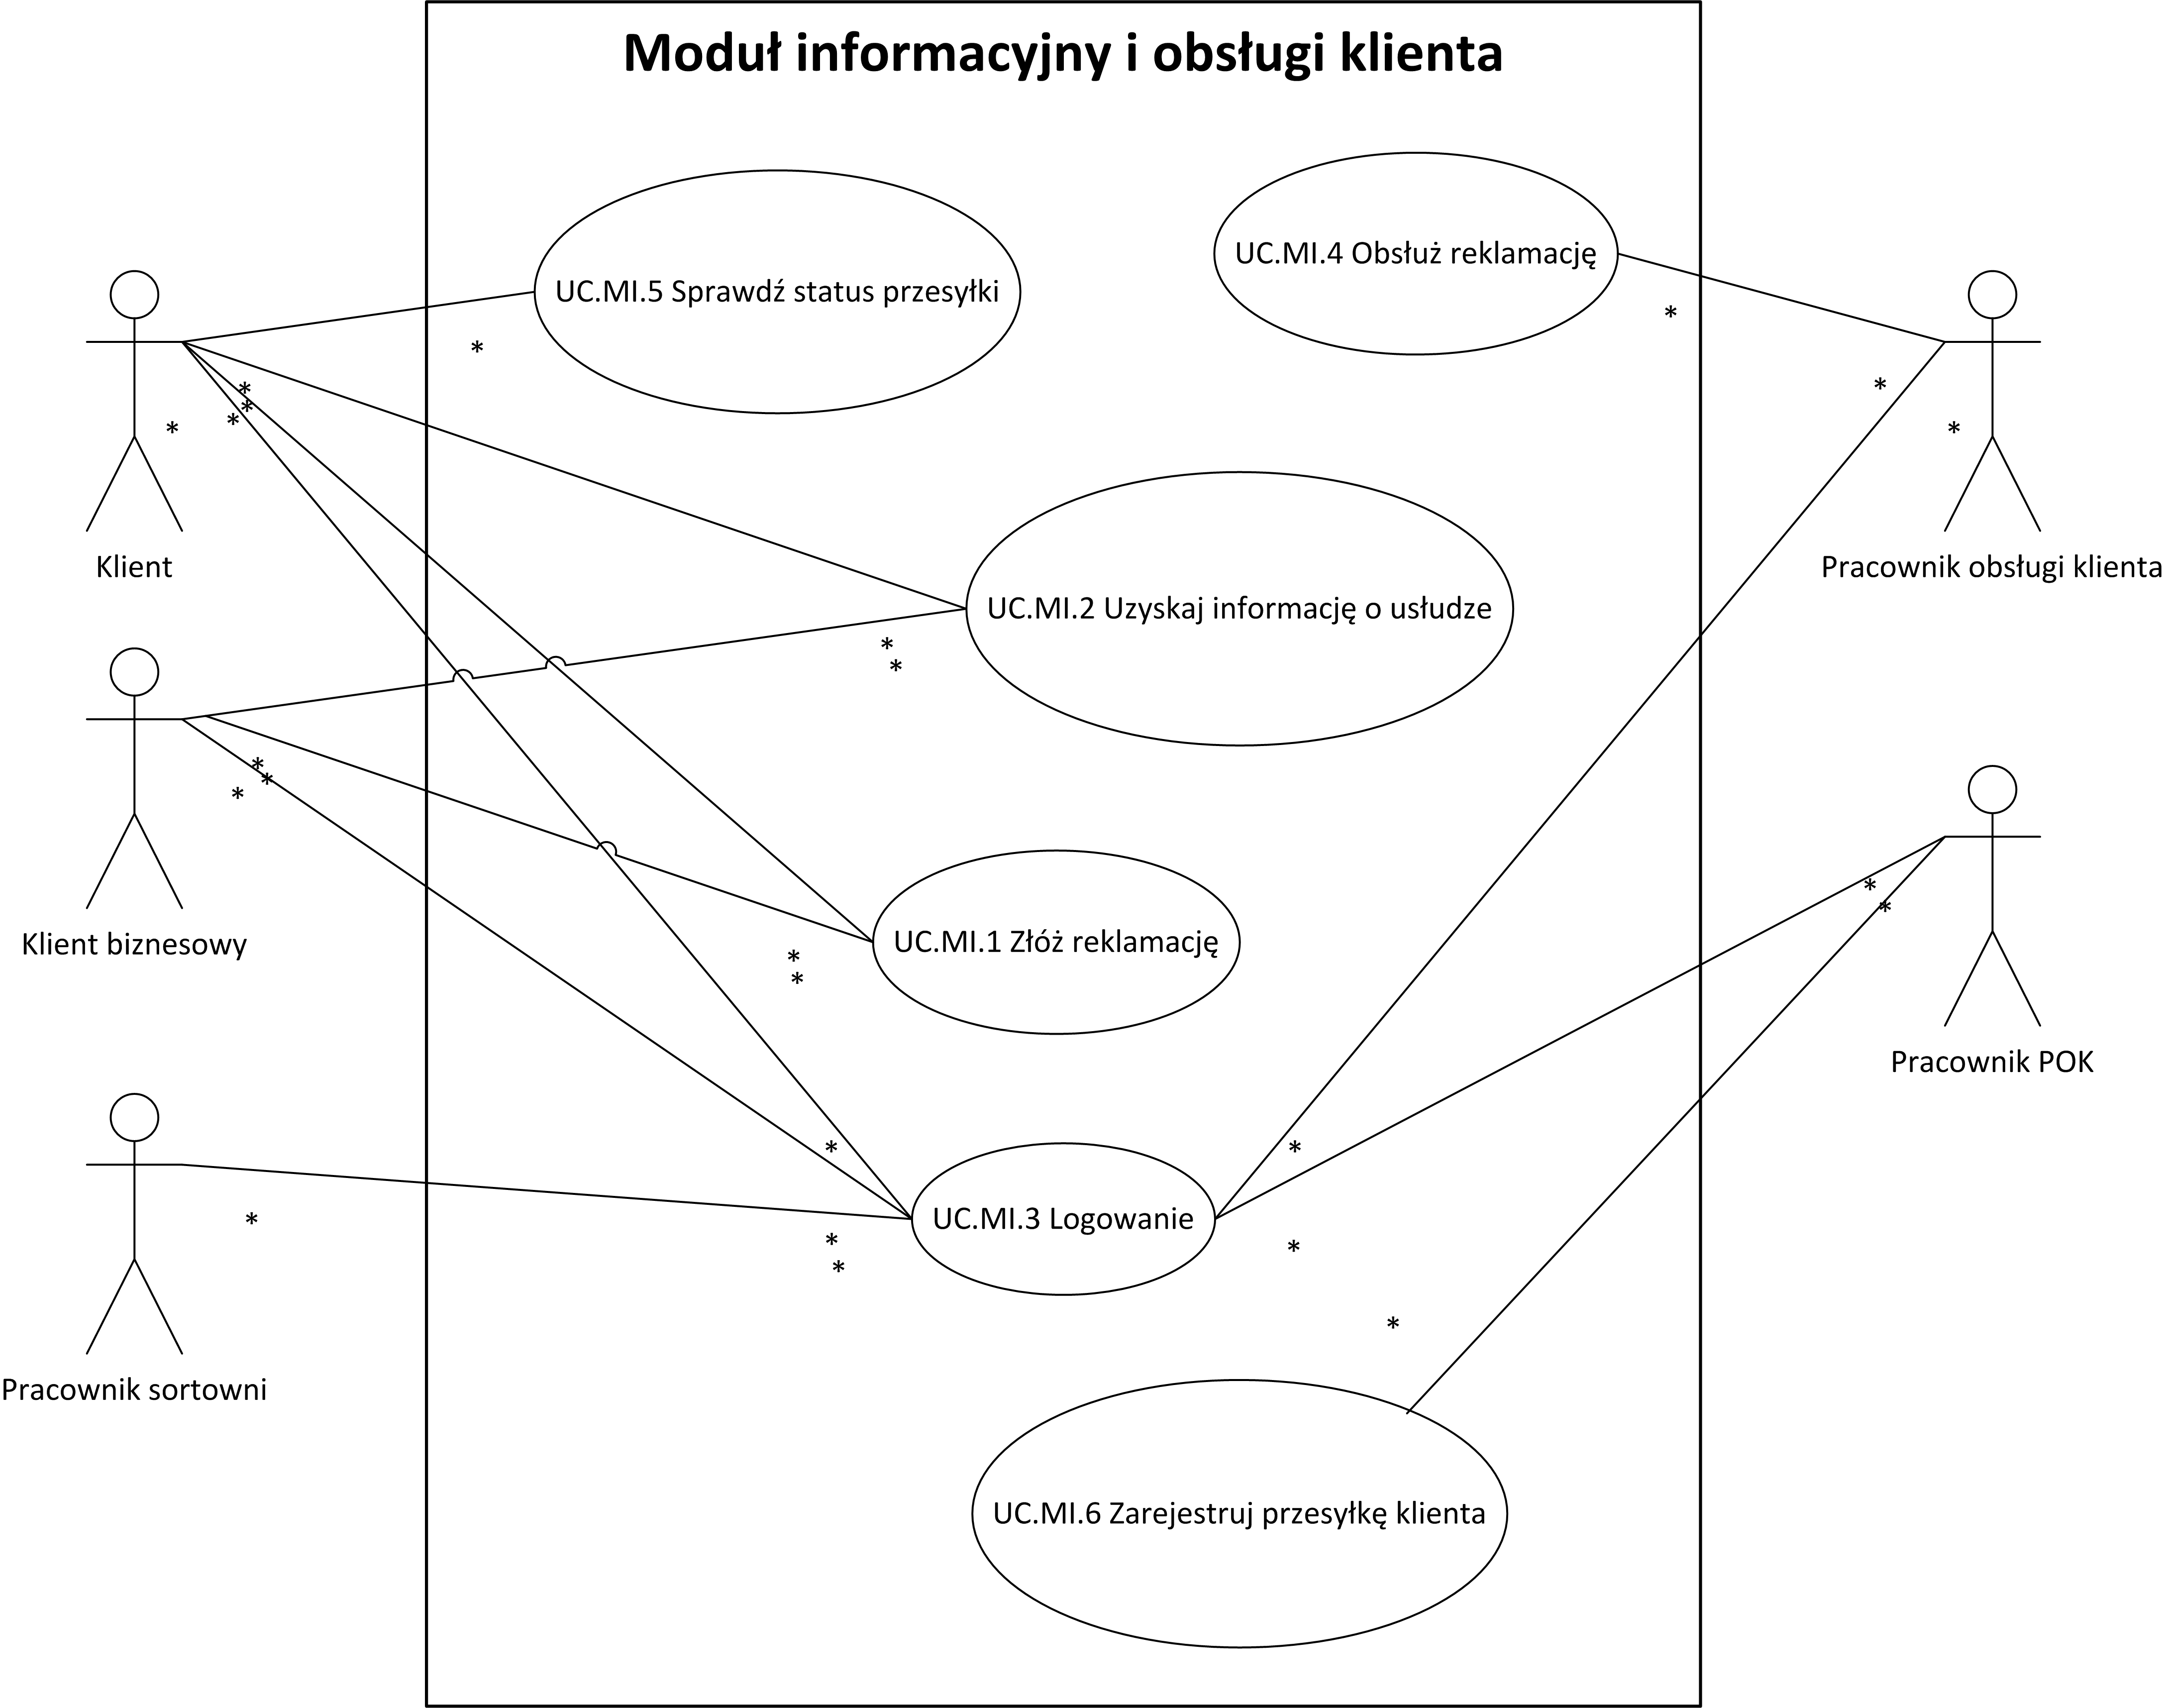
\includegraphics[width=\textwidth]{img/mod_inf_uc}
\end{figure}

\subsubsection*{Scenariusze przypadków użycia}
\begin{center}
\begin{longtable}[h]{|p{1.6cm}|p{13.5cm}|}
\hline
\textbf{ID:} & UC.MI.1 \\ \hline
\textbf{Nazwa:} & Złóż reklamację \\ \hline
\multicolumn{2}{|p{15.1cm}|}{\textbf{Aktorzy główni:} Klient lub Klient biznesowy} \\
\multicolumn{2}{|p{15.1cm}|}{\textbf{Aktorzy pomocniczy:}
\textit{brak}} \\
\multicolumn{2}{|p{15.1cm}|}{\textbf{Poziom:} Użytkownika} \\
\multicolumn{2}{|p{15.1cm}|}{\textbf{Priorytet:} Wysoki} \\
\hline
\multicolumn{2}{|p{15.1cm}|}{\textbf{Opis:}} \\
\multicolumn{2}{|p{15.1cm}|}{
Klient lub Klient biznesowy chce złożyć reklamację na wykonanie usługi.
} \\ \hline
\multicolumn{2}{|p{15.1cm}|}{\textbf{Wyzwalacze:}} \\
\multicolumn{2}{|p{15.1cm}|}{
Aktor wybiera opcję ''Złóż reklamację'' w interfejsie internetowym.
} \\ \hline
\multicolumn{2}{|p{15.1cm}|}{\textbf{Warunki początkowe:}} \\
\multicolumn{2}{|p{15.1cm}|}{
Aktor jest zalogowany w interfejsie internetowym.
} \\ \hline
\multicolumn{2}{|p{15.1cm}|}{\textbf{Warunki końcowe:}} \\
\multicolumn{2}{|p{15.1cm}|}{
Reklamacja zostaje zarejestrowana w systemie.
} \\ \hline
\multicolumn{2}{|p{15.1cm}|}{\textbf{Scenariusz główny:}} \\
\multicolumn{2}{|p{15.1cm}|}{
\begin{enumerate}
\item Aktor wybiera opcję ''Złóż reklamację''.
\item System prezentuje formularz reklamacji.
\item System uzupełnia dane klienta w formularzu na podstawie danych konta.
\item Aktor wprowadza numery przesyłek których dotyczy reklamacja.
\item Aktor wprowadza opis reklamacji.
\item System sprawdza poprawność wprowadzonych danych.
\item System nadaje reklamacji identyfikator i zapisuje ją w systemie.
\item System wyświetla potwierdzenie złożenia reklamacji.
\end{enumerate}
} \\ \hline
\multicolumn{2}{|p{15.1cm}|}{\textbf{Scenariusze alternatywne i rozszerzenia:}} \\
\multicolumn{2}{|p{15.1cm}|}{
6.a Wprowadzone dane są niepoprawne. \newline
6.a.1 System wyświetla informacje o błędnych danych. \newline
6.a.2 Aktor poprawia wprowadzone dane. \newline
6.a.3 Powrót do punktu 6 scenariusza głównego.
} \\ \hline
\multicolumn{2}{|p{15.1cm}|}{\textbf{Wyjątki:}} \\
\multicolumn{2}{|p{15.1cm}|}{
\textit{brak}
} \\ \hline
\multicolumn{2}{|p{15.1cm}|}{\textbf{Dodatkowe wymagania:}} \\
\multicolumn{2}{|p{15.1cm}|}{
\textit{brak}
} \\
\hline
\end{longtable}
\end{center}

\begin{center}
\begin{longtable}[h]{|p{1.6cm}|p{13.5cm}|}
\hline
\textbf{ID:} & UC.MI.2 \\ \hline
\textbf{Nazwa:} & Uzyskaj informacje o usłudze \\ \hline
\multicolumn{2}{|p{15.1cm}|}{\textbf{Aktorzy główni:} Klient lub Klient biznesowy} \\
\multicolumn{2}{|p{15.1cm}|}{\textbf{Aktorzy pomocniczy:} 
\textit{brak}} \\
\multicolumn{2}{|p{15.1cm}|}{\textbf{Poziom:} Użytkownika} \\
\multicolumn{2}{|p{15.1cm}|}{\textbf{Priorytet:} Wysoki} \\
\hline
\multicolumn{2}{|p{15.1cm}|}{\textbf{Opis:}} \\
\multicolumn{2}{|p{15.1cm}|}{
Aktor chce uzyskać informację o usłudze dostarczanej przez Firmę Kurierską.
} \\ \hline
\multicolumn{2}{|p{15.1cm}|}{\textbf{Wyzwalacze:}} \\
\multicolumn{2}{|p{15.1cm}|}{
Aktor przechodzi do menu ''Informacje'' interfejsu internetowego.
} \\ \hline
\multicolumn{2}{|p{15.1cm}|}{\textbf{Warunki początkowe:}} \\
\multicolumn{2}{|p{15.1cm}|}{
\textit{brak}
} \\ \hline
\multicolumn{2}{|p{15.1cm}|}{\textbf{Warunki końcowe:}} \\
\multicolumn{2}{|p{15.1cm}|}{
System prezentuje informacje o wybranej usłudze.
} \\ \hline
\multicolumn{2}{|p{15.1cm}|}{\textbf{Scenariusz główny:}} \\
\multicolumn{2}{|p{15.1cm}|}{
\begin{enumerate}
\item Aktor przechodzi do menu ''Informacje''.
\item System prezentuje listę dostępnych usług.
\item Aktor wskazuje wybraną usługę.
\item System prezentuje informacje o wybranej usłudze.
\end{enumerate}
} \\ \hline
\multicolumn{2}{|p{15.1cm}|}{\textbf{Scenariusze alternatywne i rozszerzenia:}} \\
\multicolumn{2}{|p{15.1cm}|}{
\textit{brak}} \\ \hline
\multicolumn{2}{|p{15.1cm}|}{\textbf{Wyjątki:}} \\
\multicolumn{2}{|p{15.1cm}|}{
\textit{brak}
} \\ \hline
\multicolumn{2}{|p{15.1cm}|}{\textbf{Dodatkowe wymagania:}} \\
\multicolumn{2}{|p{15.1cm}|}{
\textit{brak}
} \\
\hline
\end{longtable}
\end{center}

\begin{center}
\begin{longtable}[h]{|p{1.6cm}|p{13.5cm}|}
\hline
\textbf{ID:} & UC.MI.3 \\ \hline
\textbf{Nazwa:} & Logowanie \\ \hline
\multicolumn{2}{|p{15.1cm}|}{\textbf{Aktorzy główni:} Klient lub Klient biznesowy lub Pracownik sortowni lub Pracownik obsługi klienta lub Pracownik POK} \\
\multicolumn{2}{|p{15.1cm}|}{\textbf{Aktorzy pomocniczy:} 
\textit{brak}} \\
\multicolumn{2}{|p{15.1cm}|}{\textbf{Poziom:} Użytkownika} \\
\multicolumn{2}{|p{15.1cm}|}{\textbf{Priorytet:} Wysoki} \\
\hline
\multicolumn{2}{|p{15.1cm}|}{\textbf{Opis:}} \\
\multicolumn{2}{|p{15.1cm}|}{
Aktor chce się zalogować do jednego z interfejsów SWPFK.
} \\ \hline
\multicolumn{2}{|p{15.1cm}|}{\textbf{Wyzwalacze:}} \\
\multicolumn{2}{|p{15.1cm}|}{
Wybranie opcji ''Zaloguje'' w jednym z interfejsów SWPFK.
} \\ \hline
\multicolumn{2}{|p{15.1cm}|}{\textbf{Warunki początkowe:}} \\
\multicolumn{2}{|p{15.1cm}|}{
Aktor posiada dane do logowania w systemie.
} \\ \hline
\multicolumn{2}{|p{15.1cm}|}{\textbf{Warunki końcowe:}} \\
\multicolumn{2}{|p{15.1cm}|}{
Aktor zostaje zalogowany oraz zostaje utworzona nowa sesja w systemie.
} \\ \hline
\multicolumn{2}{|p{15.1cm}|}{\textbf{Scenariusz główny:}} \\
\multicolumn{2}{|p{15.1cm}|}{
\begin{enumerate}
\item Aktor wybiera opcję ''Zaloguj''.
\item System prezentuje formularz logowania.
\item Aktor wprowadza Identyfikator oraz Hasło.
\item System sprawdza poprawność danych.
\item System loguje użytkownika w systemie.
\item System prezentuje informacje o pomyślnym zalogowaniu.
\end{enumerate}
} \\ \hline
\multicolumn{2}{|p{15.1cm}|}{\textbf{Scenariusze alternatywne i rozszerzenia:}} \\
\multicolumn{2}{|p{15.1cm}|}{
4.a Wprowadzone dane są niepoprawne. \newline
4.a.1 System prezentuje informacje o niepoprawnych danych logowania. \newline
4.a.2 Aktor poprawia wprowadzone dane. \newline
4.a.3 Powrót do punktu 4 scenariusza głównego.
} \\ \hline
\multicolumn{2}{|p{15.1cm}|}{\textbf{Wyjątki:}} \\
\multicolumn{2}{|p{15.1cm}|}{
\textit{brak}
} \\ \hline
\multicolumn{2}{|p{15.1cm}|}{\textbf{Dodatkowe wymagania:}} \\
\multicolumn{2}{|p{15.1cm}|}{
\textit{brak}
} \\
\hline
\end{longtable}
\end{center}

\begin{center}
\begin{longtable}[h]{|p{1.6cm}|p{13.5cm}|}
\hline
\textbf{ID:} & UC.MI.4 \\ \hline
\textbf{Nazwa:} & Obsłuż reklamację \\ \hline
\multicolumn{2}{|p{15.1cm}|}{\textbf{Aktorzy główni:} ID lub nazwy aktorów głównych biorących udział w procesie} \\
\multicolumn{2}{|p{15.1cm}|}{\textbf{Aktorzy pomocniczy:} ID lub nazwy aktorów pomocniczych biorących udział w procesie} \\
\multicolumn{2}{|p{15.1cm}|}{\textbf{Poziom:}  Biznesowy / Użytkownika / Podfunkcji} \\
\multicolumn{2}{|p{15.1cm}|}{\textbf{Priorytet:}  Niski / Średni / Wysoki} \\
\hline
\multicolumn{2}{|p{15.1cm}|}{\textbf{Opis:}} \\
\multicolumn{2}{|p{15.1cm}|}{Opis procesu biznesowego.
} \\ \hline
\multicolumn{2}{|p{15.1cm}|}{\textbf{Wyzwalacze:}} \\
\multicolumn{2}{|p{15.1cm}|}{Wyszczególnienie zdarzeń wyzwalających proces.
} \\ \hline
\multicolumn{2}{|p{15.1cm}|}{\textbf{Warunki początkowe:}} \\
\multicolumn{2}{|p{15.1cm}|}{Warunki początkowe procesu.
} \\ \hline
\multicolumn{2}{|p{15.1cm}|}{\textbf{Warunki końcowe:}} \\
\multicolumn{2}{|p{15.1cm}|}{Warunki końcowe procesu.
} \\ \hline
\multicolumn{2}{|p{15.1cm}|}{\textbf{Scenariusz główny:}} \\
\multicolumn{2}{|p{15.1cm}|}{Scenariusz główny procesu.
} \\ \hline
\multicolumn{2}{|p{15.1cm}|}{\textbf{Scenariusze alternatywne i rozszerzenia:}} \\
\multicolumn{2}{|p{15.1cm}|}{Scenariusze alternatywne procesu.
} \\ \hline
\multicolumn{2}{|p{15.1cm}|}{\textbf{Wyjątki:}} \\
\multicolumn{2}{|p{15.1cm}|}{Wyjątki procesu.
} \\ \hline
\multicolumn{2}{|p{15.1cm}|}{\textbf{Dodatkowe wymagania:}} \\
\multicolumn{2}{|p{15.1cm}|}{Dodatkowe wymagania procesu.
} \\
\hline
\end{longtable}
\end{center}

\begin{center}
\begin{longtable}[h]{|p{1.6cm}|p{13.5cm}|}
\hline
\textbf{ID:} & UC.MI.5 \\ \hline
\textbf{Nazwa:} & Sprawdź status przesyłki \\ \hline
\multicolumn{2}{|p{15.1cm}|}{\textbf{Aktorzy główni:} Klient} \\
\multicolumn{2}{|p{15.1cm}|}{\textbf{Aktorzy pomocniczy:} 
\textit{brak}} \\
\multicolumn{2}{|p{15.1cm}|}{\textbf{Poziom:} Użytkownika} \\
\multicolumn{2}{|p{15.1cm}|}{\textbf{Priorytet:} Średni} \\
\hline
\multicolumn{2}{|p{15.1cm}|}{\textbf{Opis:}} \\
\multicolumn{2}{|p{15.1cm}|}{
Klient chce sprawdzić status przesyłki.
} \\ \hline
\multicolumn{2}{|p{15.1cm}|}{\textbf{Wyzwalacze:}} \\
\multicolumn{2}{|p{15.1cm}|}{
Aktor wybiera opcję ''Sprawdź status przesyłki'' w interfejsie internetowym.
} \\ \hline
\multicolumn{2}{|p{15.1cm}|}{\textbf{Warunki początkowe:}} \\
\multicolumn{2}{|p{15.1cm}|}{
Aktor posiada numer przesyłki, której status chce sprawdzić.
} \\ \hline
\multicolumn{2}{|p{15.1cm}|}{\textbf{Warunki końcowe:}} \\
\multicolumn{2}{|p{15.1cm}|}{
System prezentuje status przesyłki.
} \\ \hline
\multicolumn{2}{|p{15.1cm}|}{\textbf{Scenariusz główny:}} \\
\multicolumn{2}{|p{15.1cm}|}{
\begin{enumerate}
\item Aktor wybiera opcję ''Sprawdź status przesyłki''.
\item System prezentuje formularz do wprowadzenia numeru przesyłki.
\item Aktor wprowadza numer przesyłki.
\item System wyszukuje status przesyłki o podanym numerze.
\item System prezentuje status przesyłki.
\end{enumerate}
} \\ \hline
\multicolumn{2}{|p{15.1cm}|}{\textbf{Scenariusze alternatywne i rozszerzenia:}} \\
\multicolumn{2}{|p{15.1cm}|}{
4.a Wprowadzony numer przesyłki jest niepoprawny. \newline
4.a.1 System prezentuje informacje o niepoprawnym numerze przesyłki. \newline
4.a.2 Aktor ponownie wprowadza numer przesyłki. \newline
4.a.3 Powrót do punktu 4 scenariusza głównego. \newline
} \\ \hline
\multicolumn{2}{|p{15.1cm}|}{\textbf{Wyjątki:}} \\
\multicolumn{2}{|p{15.1cm}|}{
\textit{brak}
} \\ \hline
\multicolumn{2}{|p{15.1cm}|}{\textbf{Dodatkowe wymagania:}} \\
\multicolumn{2}{|p{15.1cm}|}{
\textit{brak}
} \\
\hline
\end{longtable}
\end{center}

\begin{center}
\begin{longtable}[h]{|p{1.6cm}|p{13.5cm}|}
\hline
\textbf{ID:} & UC.MI.6 \\ \hline
\textbf{Nazwa:} & Zarejestruj przesyłkę klienta \\ \hline
\multicolumn{2}{|p{15.1cm}|}{\textbf{Aktorzy główni:} Pracownik POK} \\
\multicolumn{2}{|p{15.1cm}|}{\textbf{Aktorzy pomocniczy:} Klient} \\
\multicolumn{2}{|p{15.1cm}|}{\textbf{Poziom:} Użytkownika} \\
\multicolumn{2}{|p{15.1cm}|}{\textbf{Priorytet:} Średni} \\
\hline
\multicolumn{2}{|p{15.1cm}|}{\textbf{Opis:}} \\
\multicolumn{2}{|p{15.1cm}|}{
Pracownik POK chce zarejestrować przesyłkę przyniesioną przez Klienta.
} \\ \hline
\multicolumn{2}{|p{15.1cm}|}{\textbf{Wyzwalacze:}} \\
\multicolumn{2}{|p{15.1cm}|}{
Klient przychodzi do POK w celu wysłania przesyłki.
} \\ \hline
\multicolumn{2}{|p{15.1cm}|}{\textbf{Warunki początkowe:}} \\
\multicolumn{2}{|p{15.1cm}|}{
Aktor jest zalogowany w aplikacji klienckiej.
} \\ \hline
\multicolumn{2}{|p{15.1cm}|}{\textbf{Warunki końcowe:}} \\
\multicolumn{2}{|p{15.1cm}|}{
Przesyłka zostaje zarejestrowana w systemie i zostaje jej nadany numer.
} \\ \hline
\multicolumn{2}{|p{15.1cm}|}{\textbf{Scenariusz główny:}} \\
\multicolumn{2}{|p{15.1cm}|}{
\begin{enumerate}
\item Aktor wybiera opcję ''Zarejestruj przesyłkę'' w menu aplikacji klienckiej.
\item System prezentuje formularz rejestrowania przesyłki.
\item Aktor wprowadza dane nadawcy oraz odbiorcy.
\item Aktor wprowadza parametry przesyłki, takie jak wymiary i waga.
\item Aplikacja kliencka przesyła do modułu serwerowego żądanie zarejestrowania przesyłki.
\item Moduł serwerowy nadaje przesyłce unikalny numer oraz rejestruje ją w systemie.
\item Moduł serwerowy przesyła potwierdzenie zarejestrowania przesyłki.
\item Aplikacja kliencka prezentuje potwierdzenie zarejestrowania.
\item Aktor wybiera opcję ''Drukuj potwierdzenie''.
\item Aplikacja kliencka przesyła żądanie drukowania do drukarki.
\end{enumerate}
} \\ \hline
\multicolumn{2}{|p{15.1cm}|}{\textbf{Scenariusze alternatywne i rozszerzenia:}} \\
\multicolumn{2}{|p{15.1cm}|}{

} \\ \hline
\multicolumn{2}{|p{15.1cm}|}{\textbf{Wyjątki:}} \\
\multicolumn{2}{|p{15.1cm}|}{
Aplikacja kliencka nie ma połączenia z modułem serwerowym.
} \\ \hline
\multicolumn{2}{|p{15.1cm}|}{\textbf{Dodatkowe wymagania:}} \\
\multicolumn{2}{|p{15.1cm}|}{
Aplikacja kliencka ma dostęp do drukarki.
} \\
\hline
\end{longtable}
\end{center}

\subsection{Obsługa doręczeń i odbiorów}
\subsubsection*{Opis}
Moduł zawiera funkcjonalności związane z bezpośrednim doręczeniem i odbiorem przesyłek od klienta.

\subsubsection*{Przypadki użycia}
\begin{figure}[H]
\centering
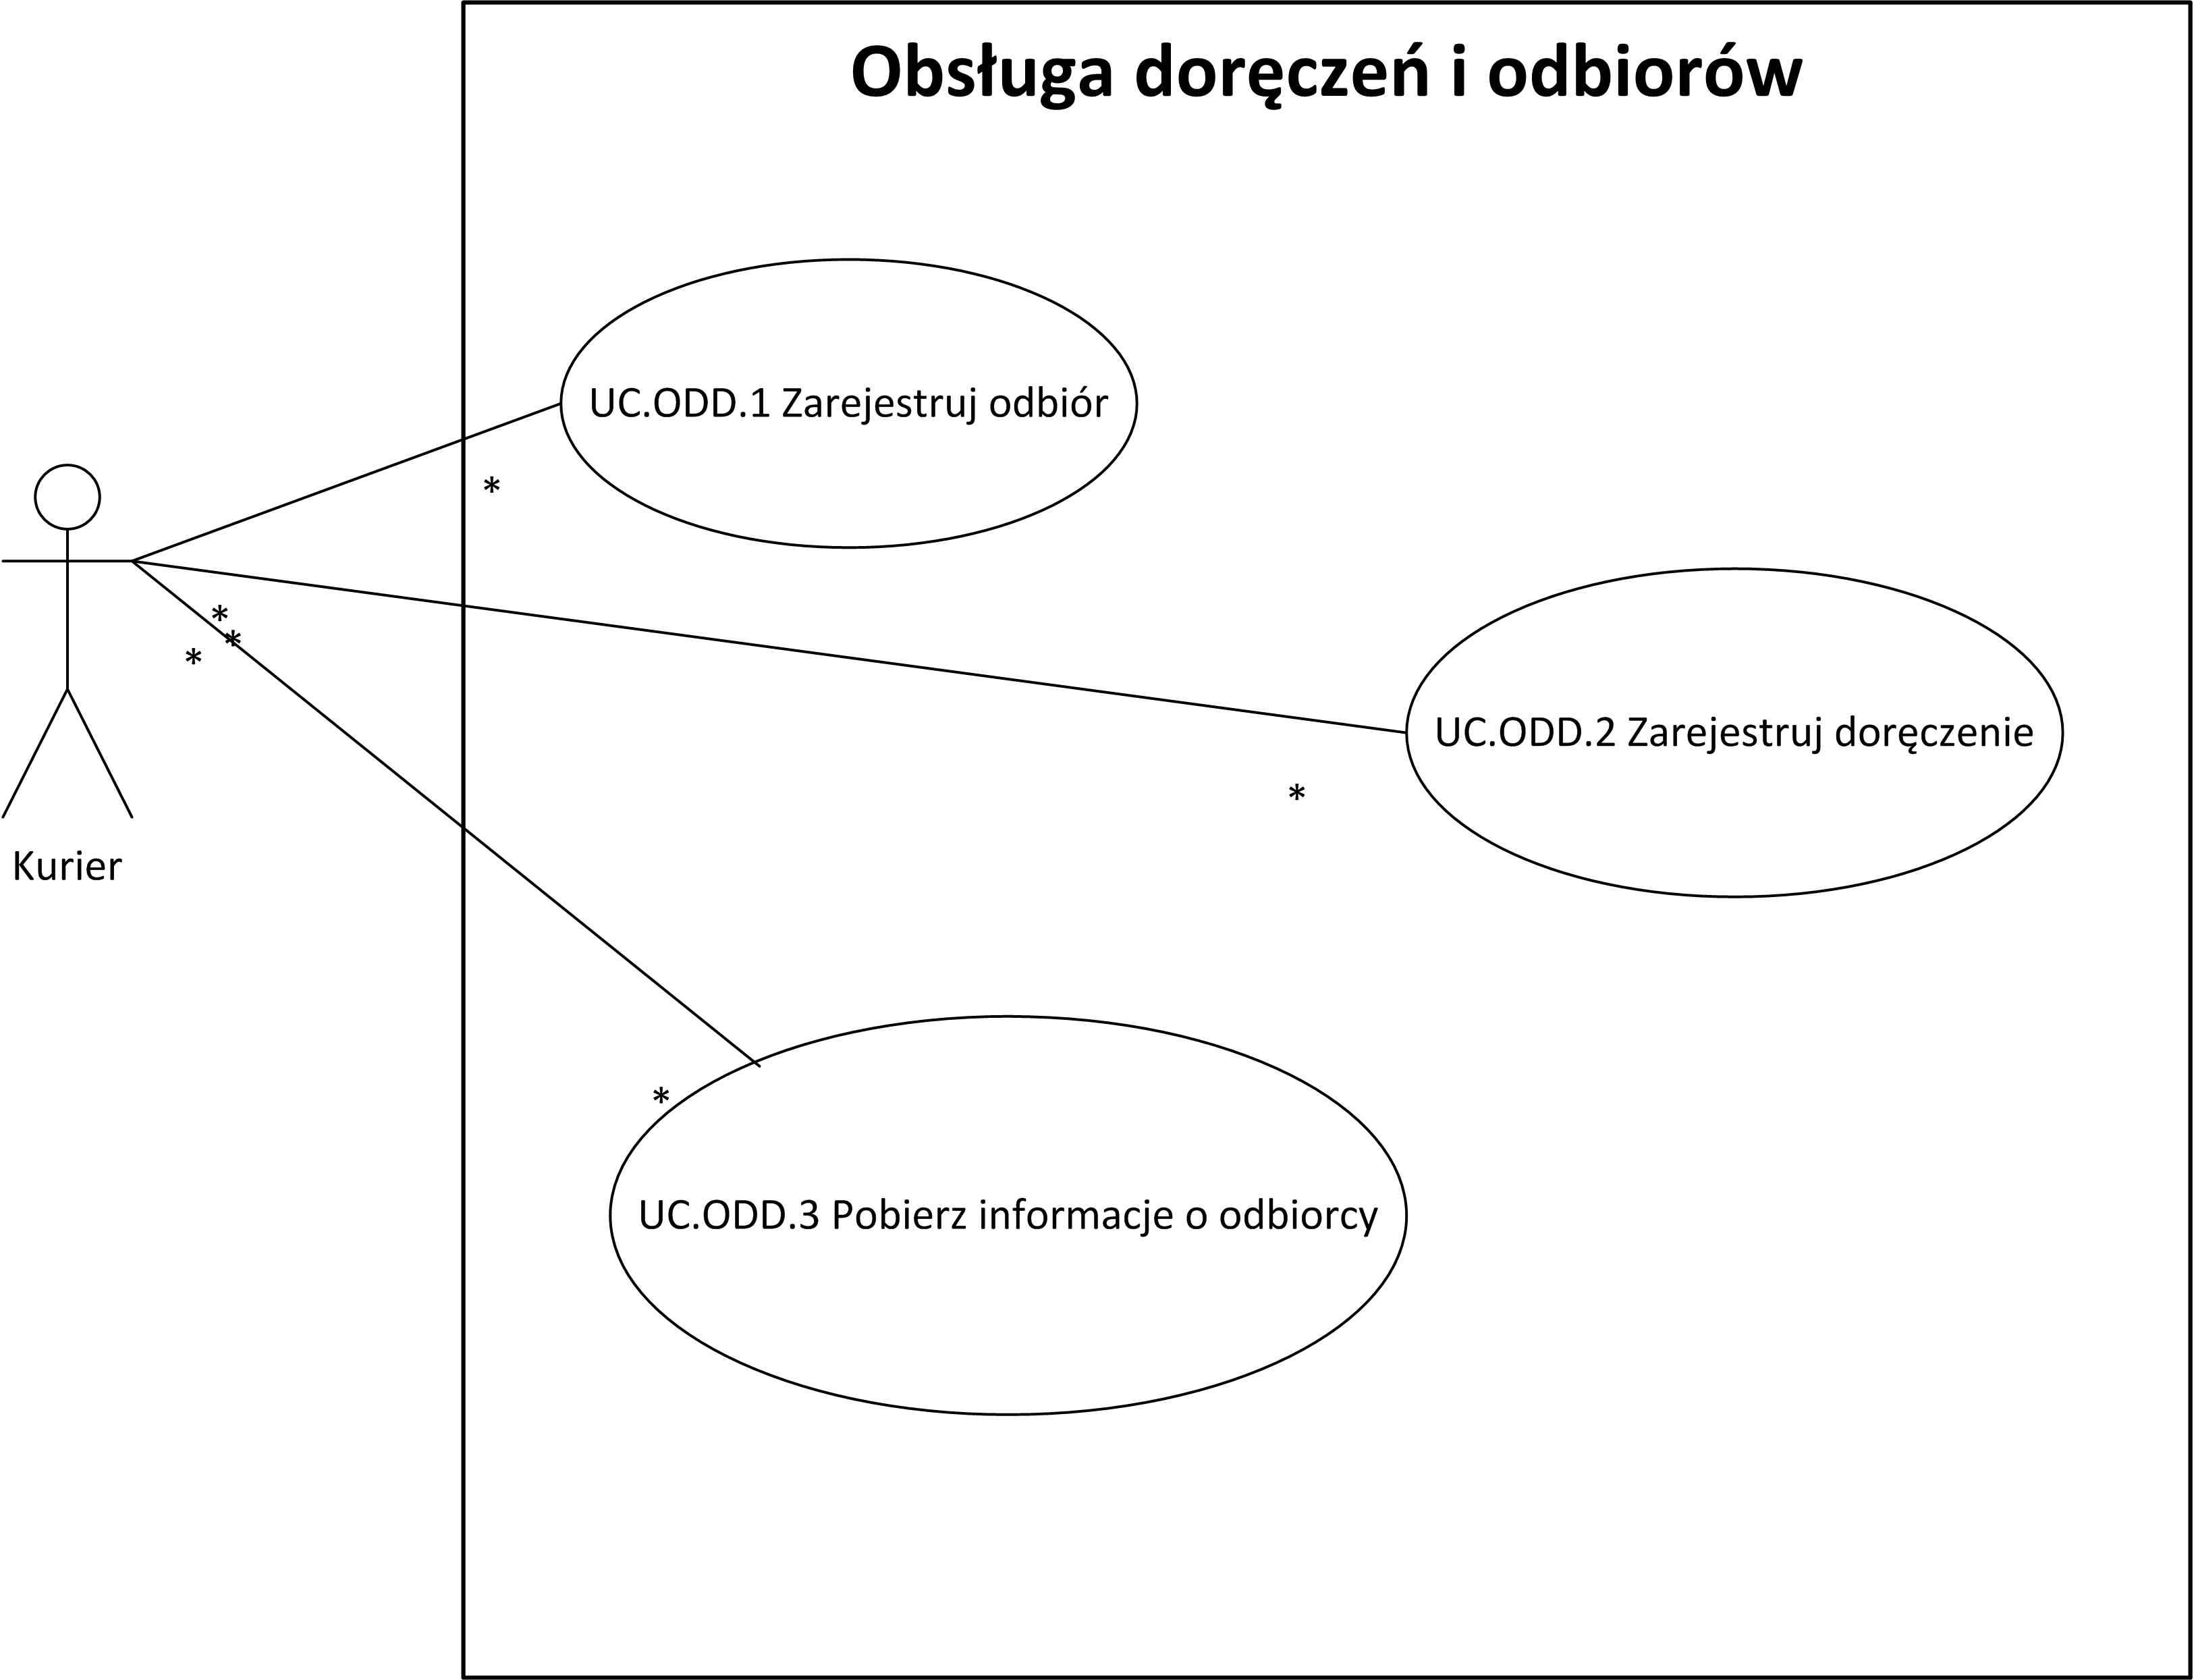
\includegraphics[width=\textwidth]{img/obs_dor_odb_uc}
\end{figure}

\subsubsection*{Scenariusze przypadków użycia}
\begin{center}
\begin{longtable}[h]{|p{1.6cm}|p{13.5cm}|}
\hline
\textbf{ID:} & UC.ODD.1 \\ \hline
\textbf{Nazwa:} & Zarejestruj odbiór \\ \hline
\multicolumn{2}{|p{15.1cm}|}{\textbf{Aktorzy główni:} Kurier} \\
\multicolumn{2}{|p{15.1cm}|}{\textbf{Aktorzy pomocniczy:} 
Klient biznesowy} \\
\multicolumn{2}{|p{15.1cm}|}{\textbf{Poziom:} Użytkownika} \\
\multicolumn{2}{|p{15.1cm}|}{\textbf{Priorytet:} Wysoki} \\
\hline
\multicolumn{2}{|p{15.1cm}|}{\textbf{Opis:}} \\
\multicolumn{2}{|p{15.1cm}|}{
Kurier chce zarejestrować odbiór przesyłki od klienta biznesowego.
} \\ \hline
\multicolumn{2}{|p{15.1cm}|}{\textbf{Wyzwalacze:}} \\
\multicolumn{2}{|p{15.1cm}|}{
Kurier odebrał przesyłki od klienta biznesowego.
} \\ \hline
\multicolumn{2}{|p{15.1cm}|}{\textbf{Warunki początkowe:}} \\
\multicolumn{2}{|p{15.1cm}|}{
Odebrane przesyłki są poprawnie oznaczone ich numerami.
} \\ \hline
\multicolumn{2}{|p{15.1cm}|}{\textbf{Warunki końcowe:}} \\
\multicolumn{2}{|p{15.1cm}|}{
Odbiór przesyłek zostaje zarejestrowany. System zmienia status przesyłek na ''Odebrane od klienta''.
} \\ \hline
\multicolumn{2}{|p{15.1cm}|}{\textbf{Scenariusz główny:}} \\
\multicolumn{2}{|p{15.1cm}|}{
\begin{enumerate}
\item Aktor wybiera opcję ''Odbiór'' w aplikacji mobilnej.
\item System aktywuje skaner kodów kreskowych terminala mobilnego.
\item Aktor skanuje kody odebranych przesyłek.
\item Po zakończeniu skanowania aktor wybiera opcję ''Zatwierdź''.
\item Aplikacja mobilna przesyła zeskanowane numery do modułu serwerowego.
\item Moduł serwerowy sprawdza przesłane numery.
\item Moduł serwerowy zmienia status podanych przesyłek na ''Odebrane od klienta''
\item Moduł serwerowy przesyła potwierdzenie powodzenia odbioru.
\item Aplikacja mobilna prezentuje potwierdzenie powodzenia.
\end{enumerate}
} \\ \hline
\multicolumn{2}{|p{15.1cm}|}{\textbf{Scenariusze alternatywne i rozszerzenia:}} \\
\multicolumn{2}{|p{15.1cm}|}{
6.a Przesłane numery przesyłek są niepoprawne. \newline
6.a.1 Moduł serwerowy przesyła informacje o błędnym numerze przesyłki. \newline
6.a.2 Aplikacja mobilna wyświetla komunikat o niepowodzeniu. \newline
6.a.3 Aktor odznacza niepoprawną przesyłkę na liście zeskanowanych numerów. \newline
6.a.4 Powrót do punktu 5 scenariusza głównego.
} \\ \hline
\multicolumn{2}{|p{15.1cm}|}{\textbf{Wyjątki:}} \\
\multicolumn{2}{|p{15.1cm}|}{
Terminal mobilny kuriera nie ma połączenia z modułem serwerowym.
} \\ \hline
\multicolumn{2}{|p{15.1cm}|}{\textbf{Dodatkowe wymagania:}} \\
\multicolumn{2}{|p{15.1cm}|}{
\textit{brak}
} \\
\hline
\end{longtable}
\end{center}

\begin{center}
\begin{longtable}[h]{|p{1.6cm}|p{13.5cm}|}
\hline
\textbf{ID:} & UC.ODD.2 \\ \hline
\textbf{Nazwa:} & Zarejestruj doręczenie \\ \hline
\multicolumn{2}{|p{15.1cm}|}{\textbf{Aktorzy główni:} Kurier} \\
\multicolumn{2}{|p{15.1cm}|}{\textbf{Aktorzy pomocniczy:} Klient lub Klient biznesowy} \\
\multicolumn{2}{|p{15.1cm}|}{\textbf{Poziom:} Użytkownika} \\
\multicolumn{2}{|p{15.1cm}|}{\textbf{Priorytet:} Wysoki} \\
\hline
\multicolumn{2}{|p{15.1cm}|}{\textbf{Opis:}} \\
\multicolumn{2}{|p{15.1cm}|}{
Kurier chce zarejestrować doręczenie przesyłek.
} \\ \hline
\multicolumn{2}{|p{15.1cm}|}{\textbf{Wyzwalacze:}} \\
\multicolumn{2}{|p{15.1cm}|}{
Klient dotarł do odbiorcy przesyłki.
} \\ \hline
\multicolumn{2}{|p{15.1cm}|}{\textbf{Warunki początkowe:}} \\
\multicolumn{2}{|p{15.1cm}|}{
Wydawane przesyłki posiadają poprawne oznaczenia. Odbiorca nie zgłasza zastrzeżeń do stanu przesyłek.
} \\ \hline
\multicolumn{2}{|p{15.1cm}|}{\textbf{Warunki końcowe:}} \\
\multicolumn{2}{|p{15.1cm}|}{
Odbiór przesyłki zostaje zarejestrowany w systemie. System zmienia status przesyłki na ''Doręczona''.
} \\ \hline
\multicolumn{2}{|p{15.1cm}|}{\textbf{Scenariusz główny:}} \\
\multicolumn{2}{|p{15.1cm}|}{
\begin{enumerate}
\item Aktor wybiera opcję ''Doręczenie'' w aplikacji mobilnej.
\item System aktywuje skaner kodów kreskowych terminala mobilnego.
\item Aktor skanuje kody wydawanych przesyłek.
\item Po zakończeniu skanowania aktor wybiera opcję ''Zatwierdź''.
\item Aplikacja mobilna umożliwia odbiorcy złożenie podpisu na ekranie dotykowym.
\item Odbiorca składa podpis w aplikacji mobilnej.
\item Aktor wprowadza imię i nazwisko odbiorcy.
\item System przesyła numery przesyłek, obraz podpisu oraz dane odbiorcy do modułu serwerowego.
\item System zmienia status przesyłek na ''Doręczona''.
\item Moduł serwerowy przesyła potwierdzenie doręczenia.
\item Aplikacja mobilna prezentuje potwierdzenie zarejestrowania odbioru.
\end{enumerate}
} \\ \hline
\multicolumn{2}{|p{15.1cm}|}{\textbf{Scenariusze alternatywne i rozszerzenia:}} \\
\multicolumn{2}{|p{15.1cm}|}{
\textit{brak}
} \\ \hline
\multicolumn{2}{|p{15.1cm}|}{\textbf{Wyjątki:}} \\
\multicolumn{2}{|p{15.1cm}|}{
Terminal mobilny kuriera nie ma połączenie z modułem serwerowym.
} \\ \hline
\multicolumn{2}{|p{15.1cm}|}{\textbf{Dodatkowe wymagania:}} \\
\multicolumn{2}{|p{15.1cm}|}{
\textit{brak}
} \\
\hline
\end{longtable}
\end{center}

\begin{center}
\begin{longtable}[h]{|p{1.6cm}|p{13.5cm}|}
\hline
\textbf{ID:} & UC.ODD.3 \\ \hline
\textbf{Nazwa:} & Pobierz informacje o odbiorcy \\ \hline
\multicolumn{2}{|p{15.1cm}|}{\textbf{Aktorzy główni:} Kurier} \\
\multicolumn{2}{|p{15.1cm}|}{\textbf{Aktorzy pomocniczy:} 
\textit{brak}} \\
\multicolumn{2}{|p{15.1cm}|}{\textbf{Poziom:} Użytkownika} \\
\multicolumn{2}{|p{15.1cm}|}{\textbf{Priorytet:} Średni} \\
\hline
\multicolumn{2}{|p{15.1cm}|}{\textbf{Opis:}} \\
\multicolumn{2}{|p{15.1cm}|}{
Kurier chce poznać dane adresowe odbiorcy przesyłki.
} \\ \hline
\multicolumn{2}{|p{15.1cm}|}{\textbf{Wyzwalacze:}} \\
\multicolumn{2}{|p{15.1cm}|}{
Aktor wybiera opcję ''Pobierz dane odbiorcy'' w aplikacji mobilnej.
} \\ \hline
\multicolumn{2}{|p{15.1cm}|}{\textbf{Warunki początkowe:}} \\
\multicolumn{2}{|p{15.1cm}|}{
\textit{brak}
} \\ \hline
\multicolumn{2}{|p{15.1cm}|}{\textbf{Warunki końcowe:}} \\
\multicolumn{2}{|p{15.1cm}|}{
System prezentuje pobrane dane adresowe odbiorcy.
} \\ \hline
\multicolumn{2}{|p{15.1cm}|}{\textbf{Scenariusz główny:}} \\
\multicolumn{2}{|p{15.1cm}|}{
\begin{enumerate}
\item Aktor wybiera opcję ''Pobierz dane odbiorcy'' w aplikacji mobilnej.
\item System aktywuje skaner kodów kreskowych terminala mobilnego.
\item Aktor skanuje kod przesyłki.
\item Aplikacja mobilna przesyła zapytania do modułu serwerowego o dane odbiorcy wraz z zeskanowanym numerem przesyłki.
\item Moduł serwerowy przesyła dane odbiorcy przesyłki.
\item Aplikacja mobilna prezentuje dane odbiorcy przesyłki.
\end{enumerate}
} \\ \hline
\multicolumn{2}{|p{15.1cm}|}{\textbf{Scenariusze alternatywne i rozszerzenia:}} \\
\multicolumn{2}{|p{15.1cm}|}{
\textit{brak}
} \\ \hline
\multicolumn{2}{|p{15.1cm}|}{\textbf{Wyjątki:}} \\
\multicolumn{2}{|p{15.1cm}|}{
Terminal mobilny kuriera nie ma połączenie z modułem serwerowym.
} \\ \hline
\multicolumn{2}{|p{15.1cm}|}{\textbf{Dodatkowe wymagania:}} \\
\multicolumn{2}{|p{15.1cm}|}{
\textit{brak}
} \\
\hline
\end{longtable}
\end{center}

\section{Charakterystyka interfejsów}

\subsection{Interfejs użytkownika}
\subsubsection{Wymagania interfejsu użytkownika}
\paragraph*{Wielojęzyczność interfejsów}
\begin{center}
\begin{tabular}[h]{|p{1.6cm}|p{13.5cm}|}
\hline
ID: & INT\_WYM\_1 \\ \hline
Nazwa: & Wielojęzyczność interfejsu użytkownika \\ \hline
Priorytet: & Wysoki \\ \hline
Opis: & Ze względu na to, że Firma Kurierska prowadzi działalność w kilku krajach Europy Środkowej oraz Zachodniej interfejsy graficzne SWPFK muszą obsługiwać języki:
\begin{itemize}
\item polski,
\item angielski,
\item niemiecki,
\item hiszpański,
\item francuski,
\item czeski,
\item słowacki.
\end{itemize} \\
\hline
\end{tabular}
\end{center}

\subsection{Interfejsy zewnętrzne}

\subsection{Interfejsy sprzętowe}

\subsection{Interfejsy programistyczne}

\subsection{Interfejsy komunikacyjne}
\section{Wymagania pozafunkcjonalne}

\subsection{Technologie}
\begin{center}
\begin{tabular}[h]{|p{1.6cm}|p{13.5cm}|}
\hline
ID: & WPF\_1 \\ \hline
Nazwa: & Wykorzystanie systemu przetwarzania danych w pamięci \\ \hline
Priorytet: & Wysoki \\ \hline
Opis: & W celu uzyskania wysokiej dostępności systemu oraz minimalizacji opóźnień przyjmuje się, że SWPFK będzie wykorzystywał system przetwarzania danych w pamięci (In-Memory Computing). Jednym z rekomendowanych rozwiązań jest oprogramowanie Gigaspace XAP. \\
\hline
\end{tabular}
\end{center}

\begin{center}
\begin{tabular}[h]{|p{1.6cm}|p{13.5cm}|}
\hline
ID: & WPF\_2 \\ \hline
Nazwa: & Technologia wykonania modułu serwerowego \\ \hline
Priorytet: & Średni \\ \hline
Opis: & Moduł serwerowy SWPFK powinien zostać wykonany w technologii Java w co najmniej 1.7, w celu zapewnienia wysokiej skalowalności aplikacji. \\
\hline
\end{tabular}
\end{center}

\begin{center}
\begin{tabular}[h]{|p{1.6cm}|p{13.5cm}|}
\hline
ID: & WPF\_3 \\ \hline
Nazwa: & Technologia wykonania interfejsu internetowego \\ \hline
Priorytet: & Średni \\ \hline
Opis: & Interfejs internetowy powinien zostać wykonany w technologii HTML oraz Java, ze względu na doświadczenie posiadane przez dział informatyczny Firmy Kurierskiej w budowie oprogramowania w tych technologiach. \\
\hline
\end{tabular}
\end{center}

\begin{center}
\begin{tabular}[h]{|p{1.6cm}|p{13.5cm}|}
\hline
ID: & WPF\_4 \\ \hline
Nazwa: & Technologia wykonania aplikacji klienckiej \\ \hline
Priorytet: & Średni \\ \hline
Opis: & Aplikacja kliencka zostanie wykonana w technologii Microsoft .NET Framework w wersji co najmniej 3.5. Technologia ta zapewni pracę aplikacji na komputerach PC pracujących pod kontrolą systemu operacyjnego Microsoft Windows oraz szerokie możliwości budowania graficznego interfejsu użytkownika. \\
\hline
\end{tabular}
\end{center}

\subsection{Wydajność}
\begin{center}
\begin{tabular}[h]{|p{1.6cm}|p{13.5cm}|}
\hline
ID: & WPF\_5 \\ \hline
Nazwa: & Wydajność usług modułu serwerowego \\ \hline
Priorytet: & Wysoki \\ \hline
Opis: & Czas wykonywania dowolnej usług w module serwerowym nie może być większy niż 300 milisekund. Czas ten jest mierzony od czasu wejścia zapytania do serwera do czasu wysłania odpowiedzi do klienta. Czasy wspomnianych akcji będą odczytywane z logów modułu serwerowego. \\
\hline
\end{tabular}
\end{center}

\begin{center}
\begin{tabular}[h]{|p{1.6cm}|p{13.5cm}|}
\hline
ID: & WPF\_6 \\ \hline
Nazwa: & Wydajność aplikacji klienckiej \\ \hline
Priorytet: & Średni \\ \hline
Opis: & Czas przejścia pomiędzy dowolnymi dwoma ekranami interfejsu aplikacji klienckiej nie może być dłuższy niż 200 milisekund. Czas jest mierzony od wywołania akcji przejścia do załadowania całości wołanego okna. Z pomiaru jest wyłączony ewentualny czas oczekiwania na odebranie odpowiedzi z usługi modułu serwerowego. \\
\hline
\end{tabular}
\end{center}

\begin{center}
\begin{tabular}[h]{|p{1.6cm}|p{13.5cm}|}
\hline
ID: & WPF\_7 \\ \hline
Nazwa: & Czas uruchamiania aplikacji klienckiej \\ \hline
Priorytet: & Niski \\ \hline
Opis: & Sumaryczny czas uruchamiania aplikacji klienckiej nie może być dłuższy niż 30 sekund. Czas ten jest mierzony od wywołania uruchomienia aplikacji do pojawienia się pełnego okna głównego aplikacji, które umożliwi użytkownikowi wykonanie dowolnej akcji. \\
\hline
\end{tabular}
\end{center}

\subsection{Niezawodność}
\begin{center}
\begin{tabular}[h]{|p{1.6cm}|p{13.5cm}|}
\hline
ID: & WPF\_8 \\ \hline
Nazwa: & Niezawodność modułu serwerowego \\ \hline
Priorytet: & Wysoki \\ \hline
Opis: & Moduł serwerowy musi charakteryzować się pełną dostępnością na poziomie 99.995\% czasu w skali miesiąca. Niedostępność modułu serwerowego definiuje się jako brak lub wygenerowanie błędnej odpowiedzi na żądania innych aplikacji i interfejsów SWPFK. Przy czym w tym przypadku do błędnej odpowiedzi nie zalicza się błędów powstałych na skutek niepoprawnej implementacji procesu biznesowego.  \\
\hline
\end{tabular}
\end{center}

\subsection{Wykorzystanie zasobów}
\begin{center}
\begin{tabular}[h]{|p{1.6cm}|p{13.5cm}|}
\hline
ID: & WPF\_9 \\ \hline
Nazwa: & Wykorzystanie pamięci RAM przez aplikację kliencką. \\ \hline
Priorytet: & Wysoki \\ \hline
Opis: & Całkowite wykorzystanie pamięci RAM w dowolnym momencie działania aplikacji klienckiej nie może przekroczyć 768 megabajtów. \\
\hline
\end{tabular}
\end{center}

\begin{center}
\begin{tabular}[h]{|p{1.6cm}|p{13.5cm}|}
\hline
ID: & WPF\_10 \\ \hline
Nazwa: & Wykorzystanie pamięci RAM podczas używania interfejsu internetowego. \\ \hline
Priorytet: & Średni \\ \hline
Opis: & Całkowite wykorzystanie pamięci RAM w dowolnym momencie korzystania z interfejsu internetowego SWPFK przez przeglądarkę internetową nie może przekroczyć 150 megabajtów. Ilość pamięci RAM jest mierzona tylko dla zakładki przeglądarki w której otwarty jest interfejs SWPFK. \\
\hline
\end{tabular}
\end{center}
\section{Inne wymagania}
Nie zdefiniowano.
\appendix
\section{Słownik pojęć i terminów}
\subsubsection*{SWPFK}
Skrót od System Wspomagania Pracy Firmy Kurierskiej. Określa całość opracowywanego systemu, na który składają się wszystkie aplikacje oraz urządzenia.

\subsubsection*{Przesyłka}
List lub paczka o określonych wymiarach oraz wadze, która została nadana przez klienta Firmy Kurierskiej w celu dostarczenie jej do określonego adresata.

\subsubsection*{Kurier}
Pracownik firmy kurierskiej zajmujący się odbieraniem oraz dostarczaniem paczek klientom.

\subsubsection*{POK}
Skrót od Punkt Obsługi Klienta, stacjonarny punkt w którym można skorzystać w niektórych usług firmy kurierskiej.

\subsubsection*{Moduł serwerowy}
Oprogramowanie uruchamiane na wyspecjalizowanym serwerze, który oferuje wysoką moc obliczeniową. Udostępnia on szereg usług z których korzystają pozostałe moduły systemu. Implementuje większość logiki biznesowej systemu.

\subsubsection*{Aplikacja kliencka}
Oprogramowanie przeznaczone do uruchomienia na komputerze klasy PC. Komunikuje się z modułem serwerowym i korzysta z jego usług za pomocą jednego z protokołów sieci Internet. Zapewnia wizualizację danych oraz możliwość ich wprowadzania do systemu.

\subsubsection*{Aplikacja mobilna}
Oprogramowanie uruchamiane na urządzeniu mobilnym, np. telefon z systemem Android, wyspecjalizowany terminal graficzny. Komunikuje się z modułem serwerowym za pomocą sieci Internet i korzysta z jego usług. Wizualizuje dane oraz zapewnia możliwość ich wprowadzania do systemu.

\subsubsection*{Interfejs internetowy}
Witryna internetowa osiągalna za pomocą przeglądarki internetowej. Wykonany za pomocą technologii HTML. Udostępniony w sieci Internet za pomocą serwera WWW.

\subsubsection*{Konto w SWPFK}
Do konta można się zalogować posiadając unikalną w skali systemu nazwę użytkownika oraz ustawione hasło. Logowanie następuje za pomocą jednego z interfejsów SWPFK. Posiadanie konta w systemie SWPFK pozwala na korzystanie z większej ilości funkcji systemu, takich jak podgląd historii nadanych przesyłek, zobowiązania z tytułu wykorzystanych usług i innych. Konto pozwala na jednoznaczną identyfikację użytkownika w systemie oraz określenie jego uprawnień.

\subsubsection*{Terminal mobilny}
Specjalne urządzenie mobilne z ekranem dotykowym posiadane przez kuriera. Zapewnia on dostęp do SWPFK za pomocą zainstalowanej na nim aplikacji mobilnej. Łączy się z siecią Internet uzyskując dostęp do SWPFK za pomocą sieci komórkowej. Posiada wbudowany skaner kodów kreskowych używany do odczytywania numeru przesyłki przedstawionego za pomocą kodu kreskowego.

\subsubsection*{Pamięć RAM}
Pamięć RAM (Random Access Memory) to pamięć operacyjna komputera PC, w której przechowywane są aktualnie uruchomione programy komputerowe.
%\section{Modele analizy}
\section{Lista spraw otwartych}
\end{document}